\pdfminorversion=4
% \documentclass[slidetop,12pt,ucs,notes=only]{beamer}
\documentclass[slidetop,12pt,ucs]{beamer}

\usepackage{ucs}
\usepackage[utf8x]{inputenc}

\usepackage{amsmath}
\usepackage{amsfonts}
\usepackage{amssymb}
\usepackage[frenchb]{babel}
\usepackage[T1]{fontenc}
\usepackage{graphicx}
\usepackage{xcolor}
\usepackage{tikz}
\usetikzlibrary{calc,shadows}
\usetikzlibrary{arrows,snakes,backgrounds}
\usetikzlibrary{fadings}
\usetikzlibrary{patterns}
\usetikzlibrary{decorations.text}
\usetikzlibrary{shapes.geometric}
\usetikzlibrary{positioning-plus}
\usetikzlibrary{node-families}
% \usepackage{gnuplot-lua-tikz}

\usepackage{multirow}

\usepackage{pslatex}

\usepackage{xspace}

\usepackage{multicol}

\usepackage{pgfpages}

\usepackage{multimedia}


% \usepackage[
% texcoord,
% grid,
% gridunit=mm,
% gridcolor=red!10,
% subgridcolor=green!10,
% ]{eso-pic}



\title{Dynamique des systèmes auto-gravitants}
\subtitle{Dynamique d'une sphère auto-gravitante isotherme et tronquée}
\author{Guillaume Plum}
\institute{Institut d'Astrophysique de Paris -- ENSTA\\Observatoire de Paris}
% \institute{Institut d'Astrophysique de Paris\\Observatoire de Paris\\ENSTA}
\date{\scriptsize{Soutenance de Thèse\\29 Septembre 2014}}

\beamertemplatetransparentcovered		 
\setbeamertemplate{blocks}[rounded][shadow=true]

\setbeameroption{show notes on second screen=right}

% \setbeameroption{hide notes}
\setbeameroption{show notes}

\usetheme{Darmstadt}
\useoutertheme{smoothbars}
\useinnertheme[shadow=true]{rounded}
\usecolortheme{orchid}
\usecolortheme{whale}

\hypersetup{
      pdfpagemode = FullScreen,%
      pdfauthor   = {Plum Guillaume},%
      pdftitle    = {Sphére isotherme et tronquée},
      pdfsubject  = {Dynamique de système auto gravitant : modèle de King, sphére isotherme en boite, ...},
      pdfkeywords = {King, sphére, isotherme, auto-gravitant, gravitant, auto},%
      pdfcreator  = {PDFLaTeX},%
      pdfproducer = {PDFLaTeX}%
}

% \AtBeginSection[]{
	% \begin{frame}{Sommaire}
		% \small \tableofcontents[currentsection, hideothersubsections]
	% \end{frame}
% }

%Définition de nouvelle commande afin de faciliter l'écriture :
\newcommand{\x}[1]{\ensuremath{#1'}} 
\newcommand{\R}{\ensuremath{\mathcal{R}}}
\newcommand{\dr}{\ensuremath{\mathrm{dr}}}
\newcommand{\dx}[1]{\ensuremath{\mathrm{d#1}}}
\newcommand{\ddp}{\ensuremath{\mathrm{dp}}}
\newcommand{\vdr}{\ensuremath{\mathrm{d}\vec{r}}}
\newcommand{\vdp}{\ensuremath{\mathrm{d}\vec{p}}}
\newcommand{\erf}{\ensuremath{\mathrm{erf}}}
\newcommand{\pint}{\displaystyle{\int}}
\newcommand{\deriv}[2]{\ensuremath{\dfrac{\mathrm{d}#1}{\mathrm{d#2}}}}
\newcommand{\King}{\textsc{King}\xspace}

\newcommand{\CH}[1]{\textsc{CH}$#1$\xspace}
\newcommand{\CHa}{\textsc{CH}$\alpha$\xspace}

\renewcommand{\(}{\ensuremath{\left(}}
\renewcommand{\)}{\ensuremath{\right)}}

\tikzset{
	basic box/.style = {
		shape = rectangle,
		align = center,
		draw = #1,
		fill = #1!25,
		rounded corners
	},
	header node/.style = {
		text depth = +0pt,
		fill = white,
		draw
	},
	header/.style = {%
		inner ysep = +1.5em,
		append after command = {
			\pgfextra{\let\TikZlastnode\tikzlastnode}
			node [header node] (header-\TikZlastnode) at (\TikZlastnode.north) {#1}
			node [span = (\TikZlastnode)(header-\TikZlastnode)]
			at (fit bounding box) (h-\TikZlastnode) {}
		}
	},
	hv/.style = {
		to path = {
			-|(\tikztotarget)\tikztonodes
		}
	},
	vh/.style = {
		to path = {
			|-(\tikztotarget)\tikztonodes
		}
	},
	fat blue line/.style = {
		ultra thick, blue
	}
}

\tikzset{
	invisible/.style = {
		opacity = 0
	},
	visible on/.style = {
		alt = {
				#1{}{invisible}
		}
	},
	alt/.code args = {
		<#1>#2#3
	}{%
		\alt<#1>{\pgfkeysalso{#2}}{\pgfkeysalso{#3}} % \pgfkeysalso doesn't change the path
	},
}

\pgfdeclareradialshading{fadingdisk}{\pgfpoint{0cm}{0cm}}{
	rgb(0cm)=(1,0,0);
	rgb(0.7cm)=(1,0,0);
	rgb(0.719cm)=(1,0,0);
	rgb(0.72cm)=(0.975,0,0);
	rgb(0.9cm)=(1,1,1)
}

\pgfdeclareradialshading{fadingdiskother}{\pgfpoint{0cm}{0cm}}{
	rgb(0cm)=(1,0,0);
	% rgb(0.3cm)=(1,0,0);
	rgb(0.15cm)=(0.975,0,0);
	% rgb(0.72cm)=(0.975,0,0);
	rgb(0.9cm)=(1,1,1)
}

\newlength\toto
\settoheight\toto{$\rho_0$, $M$, $\sigma^2$}

\begin{document}
	\begin{frame}
		\begin{titlepage}
			\begin{figure}
				\vspace{-0.5cm}
				Directeurs: Jérôme Perez et Stéphane Colombi \\
				\begin{minipage}[c]{.3\linewidth}
					\centering 
\includegraphics[scale=0.2]{Logo/logo_ENSTA.png}
				\end{minipage}
				\hfill
				\begin{minipage}[c]{.18\linewidth}
					\centering 
\includegraphics[scale=0.1]{Logo/logo-obspm.png}
				\end{minipage}
				\hfill
				\begin{minipage}[c]{.18\linewidth}
					\centering 
\includegraphics[scale=0.5]{Logo/logo-iap.png}
				\end{minipage}
			\end{figure}
		\end{titlepage}
		\note{Je vais vous présenter le travail que j'ai mené sur la dynamique des systèmes auto-gravitants, et plus précisément la dynamique d'une sphère auto-gravitante isotherme et tronquée.\par}
		\note{Ce travail a été motivé principalement par quelques faits observationnels et théorique à propos des amas d'étoiles.}
	\end{frame}
	% Faire une ou deux phrases pour le contaxte frame or not.

	\section*{Sommaire}
		\begin{frame}
			\begin{multicols}{2}
				\tableofcontents
			\end{multicols}
			\note{Nous allons commencer par expliciter certaines propriétés des SAG, puis nous enchaîneront sur les modèles utilisés pour décrire leurs états d'équilibre.  Nous aborderons alors l'étude des instabilités influençant leurs évolutions.\par}
			\note{Nous terminerons alors par l'étude de simulations mettant en scène l'évolution de ces objets.}
		\end{frame}

	\section{Propriétés des systèmes auto-gravitants}
	\begin{frame}{Sommaire}
		\small \tableofcontents[currentsection, hideothersubsections]
	\end{frame}
		\subsection{Amas globulaires}
			\begin{frame}[t]{Définition d'un amas globulaire}
				\centering 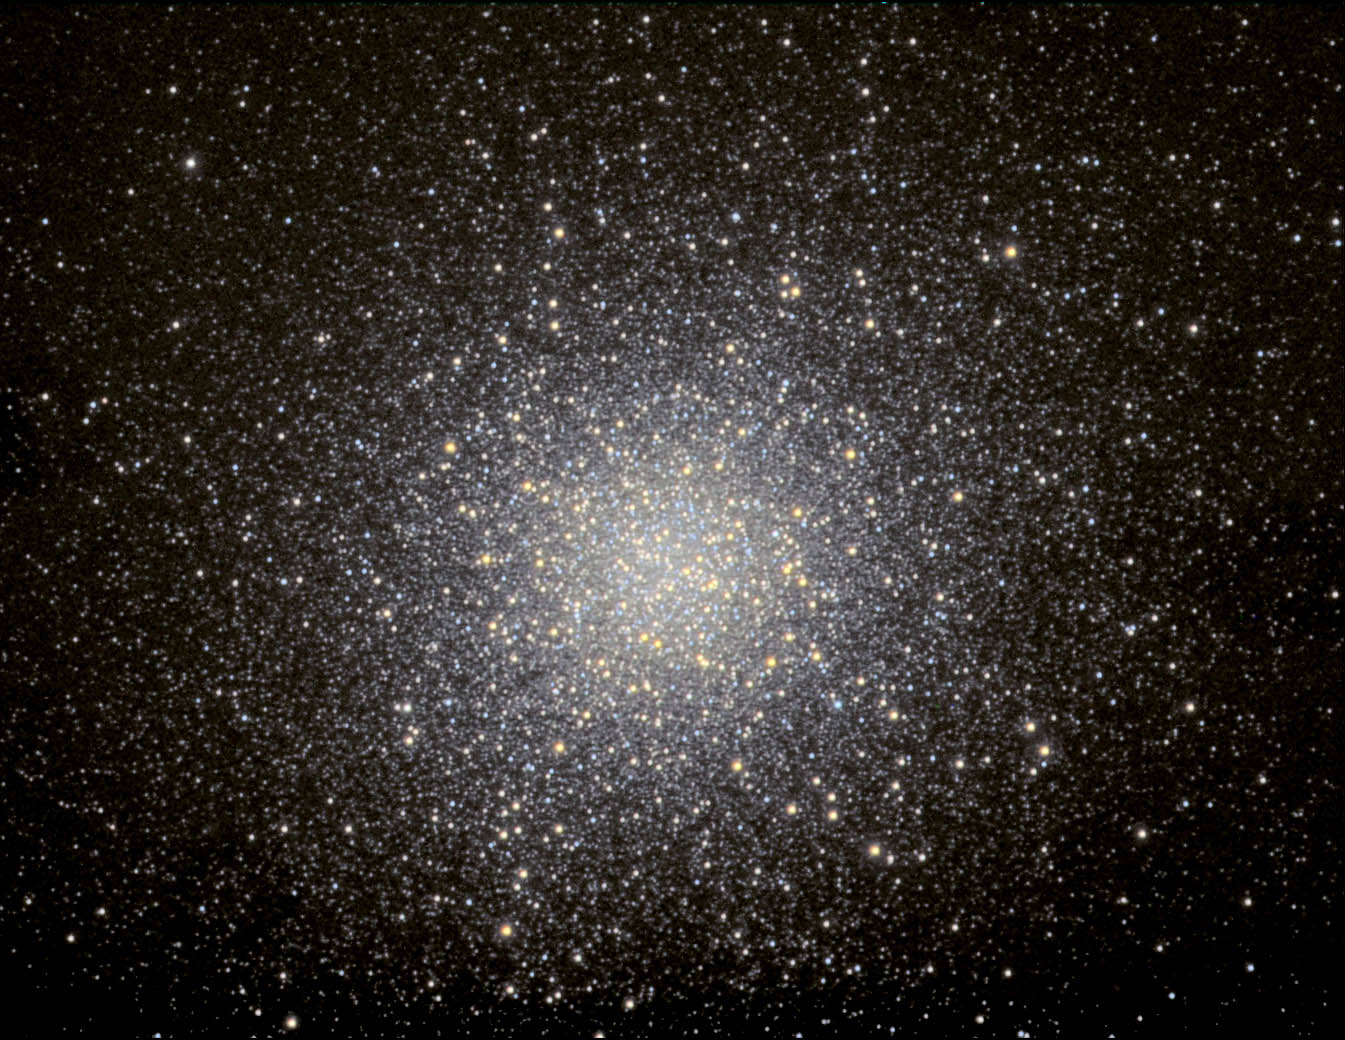
\includegraphics[width=0.85\linewidth]{M13LRGB_RC10.jpg}
				\note{C'est M13: l'amas d'hercule.\par}
				\note{Définir AG, SAG...\par}
				\note{Ag: amas d'étoile composé de de 3e4 à 1e6 étoiles, et de forme sphérique\par}
				\note{Etude montre no gaz, no dm.\par}
				\note{Notre galaxie contient plus de 140 AG.}
			\end{frame}

			\begin{frame}
				\begin{minipage}[c]{.4\linewidth}
					\begin{figure}
						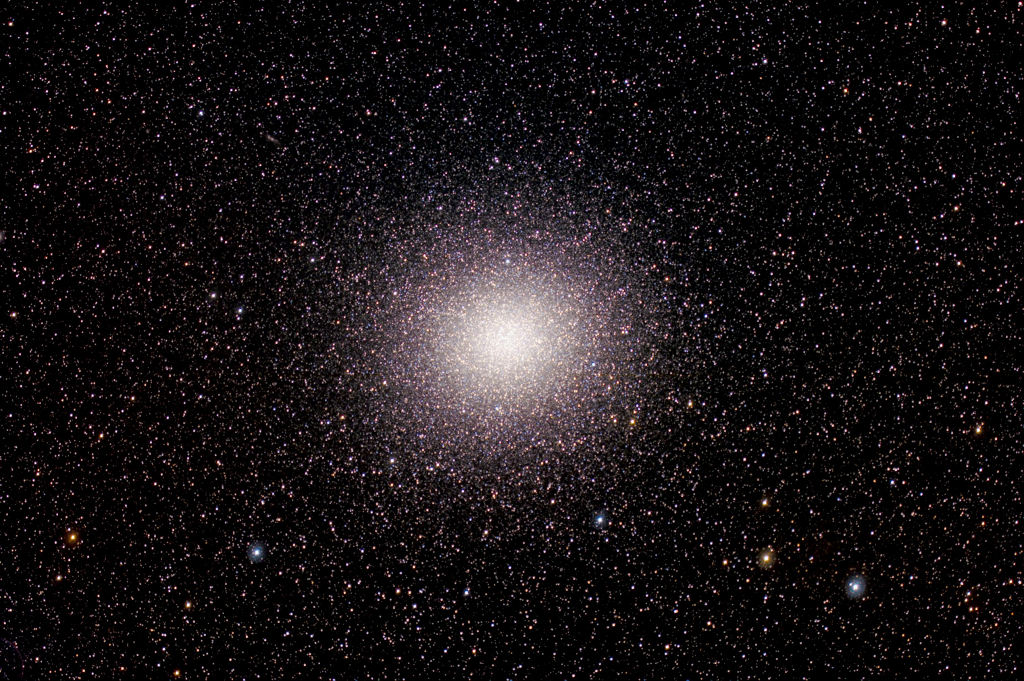
\includegraphics[scale=0.200]{graphe/ngc5139_w-cen_HD-2.png}\\$\omega$-Centauri
					\end{figure}
				\end{minipage} \hfill
				\begin{minipage}[c]{.4\linewidth}
					\begin{figure}
						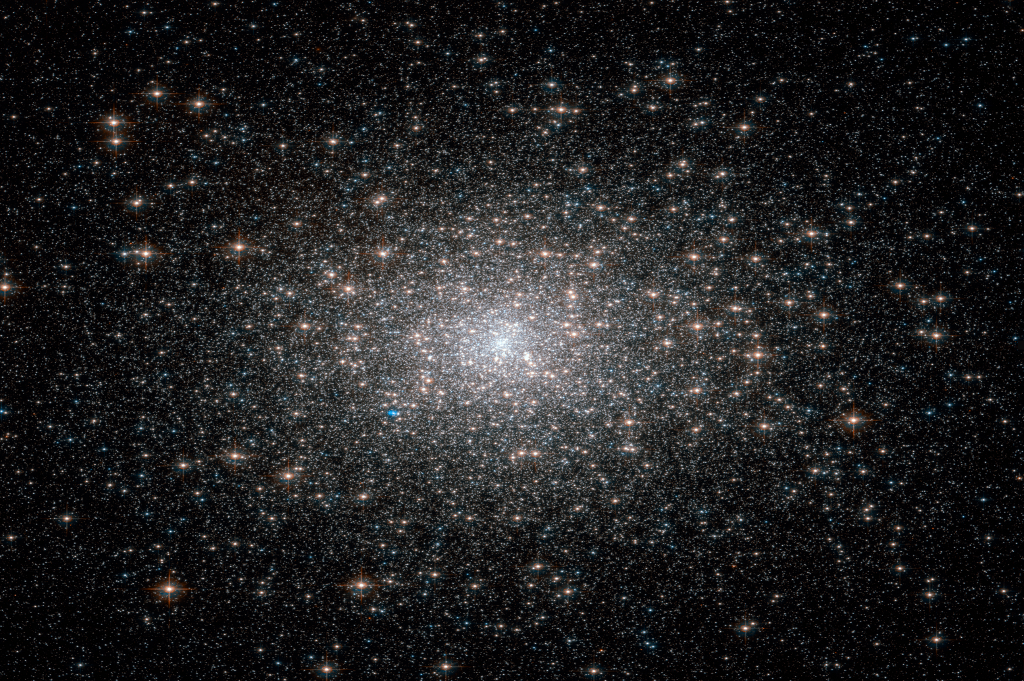
\includegraphics[scale=0.200]{graphe/m15_hst_4089_HD-2.png}\\M15
					\end{figure}
				\end{minipage}
				\note{Penser à présenter les notions de cœur et de halo sur les images\par}
				\note{Commencer par le cœur puis le halo, finir par le cœur effondré\par}
				\begin{block}{Différents états}
					\begin{itemize}
						\item $80\%$ ont une structure cœur-halo.
						\item $20\%$ présentent un cœur effondré.
					\end{itemize}
				\end{block}
				\note{amas effondre dyn plus vieux que CH.\par}

				\note{Les AG peuvent se répartir en deux états: ceux possédant une structure cœur halo. 80\% des amas globulaires sont concerné. Ils sont ici représenté par oméga du centaure.\par}
				\note{On voit sur cette image que l'AG montre une région centrale de densité centrale constante: c'est le cœur. Puis le densité d'étoile décroit: c'est le halo. Cette décroissance suit une loi de puissance.\par}
				\note{Le second état, concernant 20\% des AG, est représenté ici par M15. C'est AG sont dit cœur effondré car, lorsqu'on les observes, ils ne montrent plus de cœur! Ces AG sont dynamiquement plus vieux que les précédents.}
			\end{frame}

			\begin{frame}
				\frametitle{Profil de brillance de surface}
				\centering \emph{\scriptsize{R. Elson, P.Hut and S. Inagaki, 1987}}

				\begin{figure}
					\centering 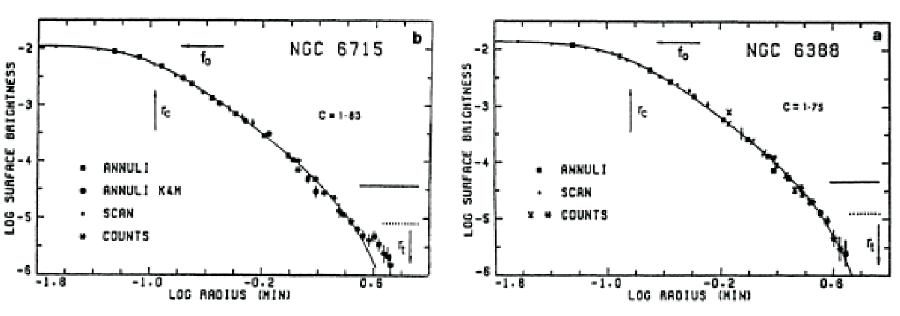
\includegraphics[scale=0.30]{graphe/Fit_King-Jerome.png}
				\end{figure}
				\note{On sait depuis les années 60 que les AG sont très bien ajusté par le modèle de King, que je détaillerai plus tard. Vous avez ici deux profils de luminosité de surface de deux amas globulaire, ajusté (en trait plein) par ce modèle.\par}
				\note{Nous voyons assez nettement la structure cœur halo sur ces graphiques.\par}

				\note{Ces différents états indique une séquence d'évolution. Nous allons essayer de vérifier cette assertion.}
			\end{frame}

			\begin{frame}[t]{Analyse de données: évolution dynamique des amas}
				\note<1>{\scriptsize Pour ce faire, nous allons nous servir de deux jeux de données. Le premier viens du catalogue de Harris. Ce catalogue recense une trentaine de paramètres observationnels, dynamiques et morphologique de tous les AG de la galaxie.
					2 paramètres nous intéressant particulièrement sont le temps dynamique: le temps mit par une étoile dans l'amas pour parcourir son orbite. Et le temps de relaxation par collision: c-à-d le temps mit par les collisions à 2
					corps à influer sur la dynamique du système}
				\note<2->{Nous récupérons ensuite les profils de brillance de surface d'une centaine d'AG de la galaxie.\par}
				\note<2->{Le problème est que c'est profils de brillance de surface nous donne une information 2D, or nous voudrions une information 3D sour la forme du profil de densité volumique de masse. Pour ce faire, nous entamons un travail
				de déprojection afin de passer de la brillance de surface à une brillance volumique puis nous utilisons les ratio masse luminosité donnés dans le catalogue pour obtenir le profil de densité. Nous en récupérons alors la pente du halo.}
				\begin{block}{Données}
					\begin{enumerate}
						\item<1-> Catalogue de Harris
						% \note[item]<1->{30aine de paramètres dynamique, morpho, observationnels... Pour tous les AG}
						\item<2-> Profil de luminosité (\emph{\scriptsize{Scott C. Trager, I. King, S. Djorgovski, 1995}})
						% \item<2-> Profil de luminosité (\emph{\scriptsize{Scott C. Trager, I. King, S. Djorgovski, Catalogue of galactic globular-cluster surface-brightness profiles, The Astronomical Journal, pp. 109-218, 1995}})
					\end{enumerate}
				\end{block}

				\begin{center}
					\large\alt<1>	{ $T_d$, $T_c \propto \dfrac{N}{\ln N} T_d$ }
					{ $I(R) \xrightarrow{\text{déprojection}} \nu(r) \xrightarrow{\Upsilon = \frac{M}{L}} \rho(r) \Rightarrow \alpha$ }
							% { $I(R) \overset{\mathrm{déprojection}}{\rightarrow} \nu(r) \rightarrow \rho(r) \Rightarrow \alpha$ }
				\end{center}
			\end{frame}

			\begin{frame}
				\frametitle{Analyse de données: évolution dynamique des amas}
				\begin{figure}
					\centering 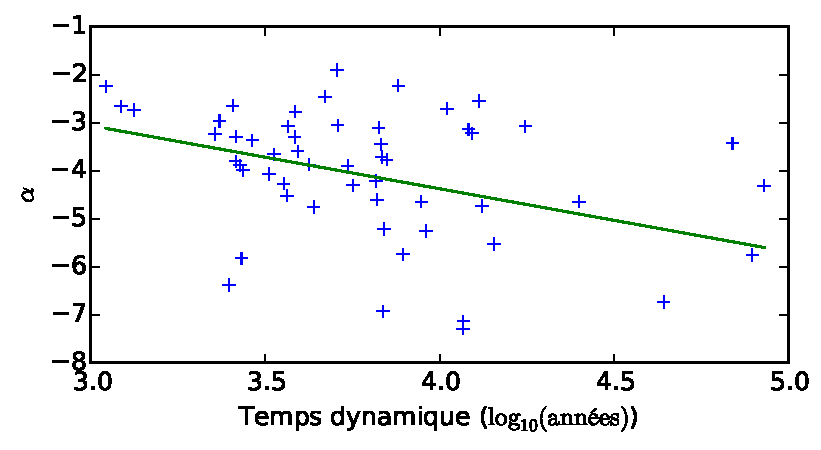
\includegraphics[width=\textwidth]{graphe/pente_tdvs.pdf}
				\end{figure}
				\note{Nous traçons alors l'évolution de cette pente en fonction du temps dynamique de l'amas. Une nette tendance apparaît alors: plus un amas est dynamiquement jeune, et est donc à droite sur le graphique, plus la pente de son halo
				est faible. Ensuite, plus il vieilli et se déplace donc vers la gauche, plus sa pente augmente, jusqu'à une valeur proche de $-2$.}
			\end{frame}

			\begin{frame}
				\frametitle{Modèle d'évolution}
				\begin{block}{Les paramètres évoluent avec l'âge dynamique}
					
	\begin{figure}[ht!]
		\begin{minipage}[b]{0.20\linewidth}
			\begin{center}
				\begin{tikzpicture}[scale=0.5]
%					Tracé de la grille :
					\draw[step=.5cm,gray,very thin] (0,0) grid (2.5,2.5);
%					Tracé des axes :
					\draw (0,0) -- (0,2.5);
					\draw (0,0) -- (2.5,0);
%					Tracé du graphe :
					\draw[red,very thick] (0,1.0) -- (1.5,1.0) -- (1.75,0);
%					\draw[red,very thick] (1.5,1.0) -- (1.75,0);
					\draw (1.75,0.5) node[right]{$r^{-4}$};
					\draw (1.25,2.5) node[above]{$t = 0$};
				\end{tikzpicture}
			\end{center}
		\end{minipage}\hfill
		\begin{minipage}[b]{0.20\linewidth}
			\begin{center}
				\begin{tikzpicture}[scale=0.5]
%					Tracé de la grille :
					\draw[step=.5cm,gray,very thin] (0,0) grid (2.5,2.5);
%					Tracé des axes :
					\draw (0,0) -- (0,2.5);
					\draw (0,0) -- (2.5,0);
%					Tracé du graphe :
					\draw[red,very thick] (0,1.5) -- (1,1.5) -- (1.5,0);
%					\draw[red,very thick] (1,1.5) -- (1.5,0);
					\draw (1.25,0.5) node[above right]{$r^{-3}$};
					\draw (1.25,2.5) node[above]{$t = 1$};
				\end{tikzpicture}
			\end{center}
		\end{minipage}\hfill
		\begin{minipage}[b]{0.24\linewidth}
			\begin{center}
				\begin{tikzpicture}[scale=0.5]
%					Tracé de la grille :
					\draw[step=.5cm,gray,very thin] (0,0) grid (2.5,2.5);
%					Tracé des axes :
					\draw (0,0) -- (0,2.5);
					\draw (0,0) -- (2.5,0);
%					Tracé du graphe :
					\draw[red,very thick] (0,2) -- (0.5,2) -- (1.5,0);
%					\draw[red,very thick] (0.5,2) -- (1.5,0);
					\draw (1,1) node[right]{$r^{-2}$};
					\draw (1.25,2.5) node[above]{$t = 2$};
				\end{tikzpicture}
			\end{center}
		\end{minipage}\hfill
		\begin{minipage}[b]{0.20\linewidth}
			\begin{center}
				\begin{tikzpicture}[scale=0.5]
%					Tracé de la grille :
					\draw[step=.5cm,gray,very thin] (0,0) grid (2.5,2.5);
%					Tracé des axes :
					\draw (0,0) -- (0,3.2);
					\draw (0,0) -- (2.5,0);
%					Tracé du graphe :
					\draw[red,very thick] (0,3) -- (1.5,0);
					\draw (1,1) node[right]{$r^{-2}$};
					\draw (1.25,2.5) node[above]{$t = \infty$};
				\end{tikzpicture}
			\end{center}
		\end{minipage}
%		\caption{Évolution d'un amas selon notre scénario\label{schema-effondrement}}
	\end{figure}


				\end{block}
				\note{\scriptsize en mettant ensemble ce que nous venons d'observer et quelque fait connu sur l'évolution des AG, notamment l'augmentation de leur densité central au cours du temps, nous construisons le scénario d'évolution suivant:\par}
				\note{Il est communément admis que les AG se sont formé à partir d'un nuage homogène qui c'est effondré sur lui-même. Les simulations numérique nous apprennent alors que ces objets nouvellement formés ont une structure de cœur halo
				de pente $-4$. Les amas évoluent alors au cours du temps en voyant leurs pentes augmenter. Dans le même temps, la densité centrale augmente et le rayon du cœur diminue. Jusqu'au moment ou le cœur s'effondre sous l'influence de
				l'instabilité d'Antonov.}
				% \note{Simu nous disent effondrement de sphère homo donne $r^{ -4 }$\par}
				% \note{Au cours du temps, densité cœur augmente, pente augmente, jusqu'à Antonov\par}
				\begin{alertblock}{Facteurs de cette évolution}
					\begin{itemize}
						\item relaxation à 2 corps
						\item perte de particules
						\item effets de marée
						\item spectre de masse des étoiles
						\item ...
					\end{itemize}
				\end{alertblock}
				\note{Les différents facteurs avancé jusqu'ici pour expliquer cette évolution sont: cité les différents facteur. Nous verrons qu'il peut y en avoir d'autre. }
				% \note{Effets...\par}
				\note{Ce scénario est en bon accord avec les observations et les simulations numériques, bien que jamais vraiment mentionné.}
			\end{frame}

		\subsection{Galaxies}

			\begin{frame}[t]{Profils}
				\begin{center}
					\begin{tikzpicture}
						\node[basic box = blue, header = de Veaucouleur (1948), anchor = north] {
								{\scriptsize$
									I(R) = I_\mathrm{eff} 10^{-3.3\left[\(\dfrac{R}{R_\mathrm{eff}}\)^{1/4} - 1\right]}
								$}
						} [sibling distance = 60mm, level distance = 35mm] child[visible on=<2->] {
							node[basic box = red, header = Einasto (1965), anchor = north] {
								{\scriptsize$
									\rho(r) = \rho_e\exp\left[-d_n\left\{\(\frac{r}{r_e}\)^{1/n} - 1\right\}\right]
								$}
							}
						} child[visible on=<3->] {
							node[basic box = red, header = Prugniel-Siemiens (1997), anchor = north] {
								{\scriptsize$
									\rho(r) = \rho_0 \(\dfrac{r}{R_e}\)^{-p_n} \exp\left[-b_n\left\{\(\frac{r}{r_e}\)^{1/n} - 1\right\}\right]
								$}
							}
						};
					\end{tikzpicture}
				\end{center}
					\note[item]<1->{Depuis observation galaxie, on peut ajuster luminosité de surface des galaxies elliptique par loi en $R^{1/4}$ de de Veaucouleur. Mais, en théorie, on a besoin théorique d'information en 3D, donc de la densité $\rho$}
					\note[item]<2->{Les premiers modèle de $\rho$ sont de simple transposition de cette loi qui a donnée un CH: Eiansto. Puis on a voulu pouvoir ajuster les autres donc deproj plus complexe}
					\note[item]<3->{C'est alors qu'on a obtenu PS qui permet d'ajuster des obj avec aussi CH que cusp.}
			\end{frame}

			\begin{frame}[t]{Halos de matière noire}
					\centering \includegraphics[width=0.55\linewidth]{aquarius.png}\\\centering Simulation Aquarius
					\begin{block}{Navarro-Franck-White (Navarro et al, 1996)}
						$$\rho(r) = \dfrac{\rho_0}{r(r+a)^2}$$
					\end{block}
					\note{Lorsque l'on parle de galaxie, nous en venons aussi aux halos de matière noire. Ces halo sont ajusté en utilisant le profil "Universel" de NFW (dire explicitement). De récentes étude montrent que les profils d'Einasto
					ajuste mieux, dans certains cas du moins, les halos de DM.\par}
					\note{\par}
					\note{Ag et Galaxies ont des de densité similaire. Bien que leurs processus de formations et d'évolutions soient différents, ce sont des SAG. L'hypothèse généralement faîte est que les SAG observé sont à dans un état d'équilibre.
						Leurs états d'équilibre sont souvent assimilé à des gaz d'étoiles et peuvent donc être décrit par la physique statistique.}
			\end{frame}

			%% Rajouter slides NFW--DM formule simu aquarius (cf slides steph)
			% Ag et galaxie: \rho similaire, mais évolution différente tout en étant piloté par grav, ce sont des sag. => thermodyn des sag. New slides: recherche du max de l'entropie -> sphère isotherme,
			% pb en l'infini m(r)=\infty

	\section{Différents modèles}
	\begin{frame}{Sommaire}
		\note{Je vais commencer par vous présenter le modèle de la sphère isotherme. J'enchainerai sur deux modèles créés pour rendre la sphère isotherme viable.}
		\small \tableofcontents[currentsection, hideothersubsections]
	\end{frame}
		\subsection{Sphère isotherme}
			\begin{frame}
				\note{Dans le cadre de la thermodynamique, l'hypothèse la plus naturelle est de chercher le maximum de l'entropie.\par}
				\frametitle{Les modèles isothermes}
				\begin{block}{Thermodynamique des systèmes auto-gravitants}
					\begin{itemize}
						\item<1->[] Équilibre $\Leftrightarrow$ Maximum de l'entropie $S = \int f \ln f$ ($f$ étant la fonction de distribution dans l'espace des phases).
							\note[item]<1->{Qui dit équilibre thermo dit max de l'entropie}
						\item<2->[$\hookrightarrow$] sphère isotherme: $f \propto e^{-\beta E}$ pour $M=cte$ et $E_t=cte$
							% Solution implique $\rho \propto r^{ -2 }$ venu de poisson car besoin résoudre potentiel
							\note[item]<2->{Avec les hypothèse de masse et d'énergie finie, on obtient la sphère isotherme: une maxwellienne.}
						\item<3->[] Après résolution de l'équation de Poisson: $\rho \propto \dfrac{1}{r^2}$
						\item<4->[$\Rightarrow$] Le système n'est pas borné spatialement: masse infinie.
						% \item<3->[] Masse infinie: $\rho \propto \dfrac{1}{r^2}$
							\note[item]<3->{Comme elle n'est pas bornée spatialement: 2 problèmes: la masse infinie.}
					\end{itemize}
				\end{block}

				\only<5->{
					\begin{alertblock}{La solution}
						Utiliser une troncature:
						\begin{itemize}
							\item Méthode empirique: Modèle de \King $f \propto e^{ \beta (E_l - E)}$
							\item Méthode théorique: la thermodynamique des systèmes auto-gravitants dans une boîte
						\end{itemize}
					\end{alertblock}
				}
			\end{frame}
		\subsection{Modèle de \King}
			\begin{frame}
				\frametitle{Modèle de \King}
				\note<1>{Ce modèle empirique ajuste très bien les AG (et les galaxies naines). Il possède 3 paramètres.}

				$$
					f_K(E) = \begin{cases}
						\rho_0 \(2\pi m\sigma^2\)^{-3/2}\( e^{\frac{E_l-E}{\sigma^2}} - 1\) & \text{si $E < E_l$} \\
						0 & \text{si $E > E_l$}
					\end{cases}
				$$

				\begin{block}{3 paramètres}
					\begin{itemize}
						\item énergie de libération: $E_l$
						\note[item]<1>{$E_l$ qui correspond à la troncature dans l'espace des phases}
						\item profondeur du puits de potentiel: $W_0$
						\note[item]<1>{Qui permet de jouer sur la profondeur du puit}
						\item rayon du cœur: $r_c$
						\note[item]<1>{pour jouer sur le rayon de cœur}
					\end{itemize}
				\end{block}
			\end{frame}
			\begin{frame}[t]{Modèle de \King}
				\begin{figure}
					\centering
					\begin{tikzpicture}[overlay]
						\node at ($(current page.north west) + (0.0\paperwidth, -1.2\paperheight)$) { 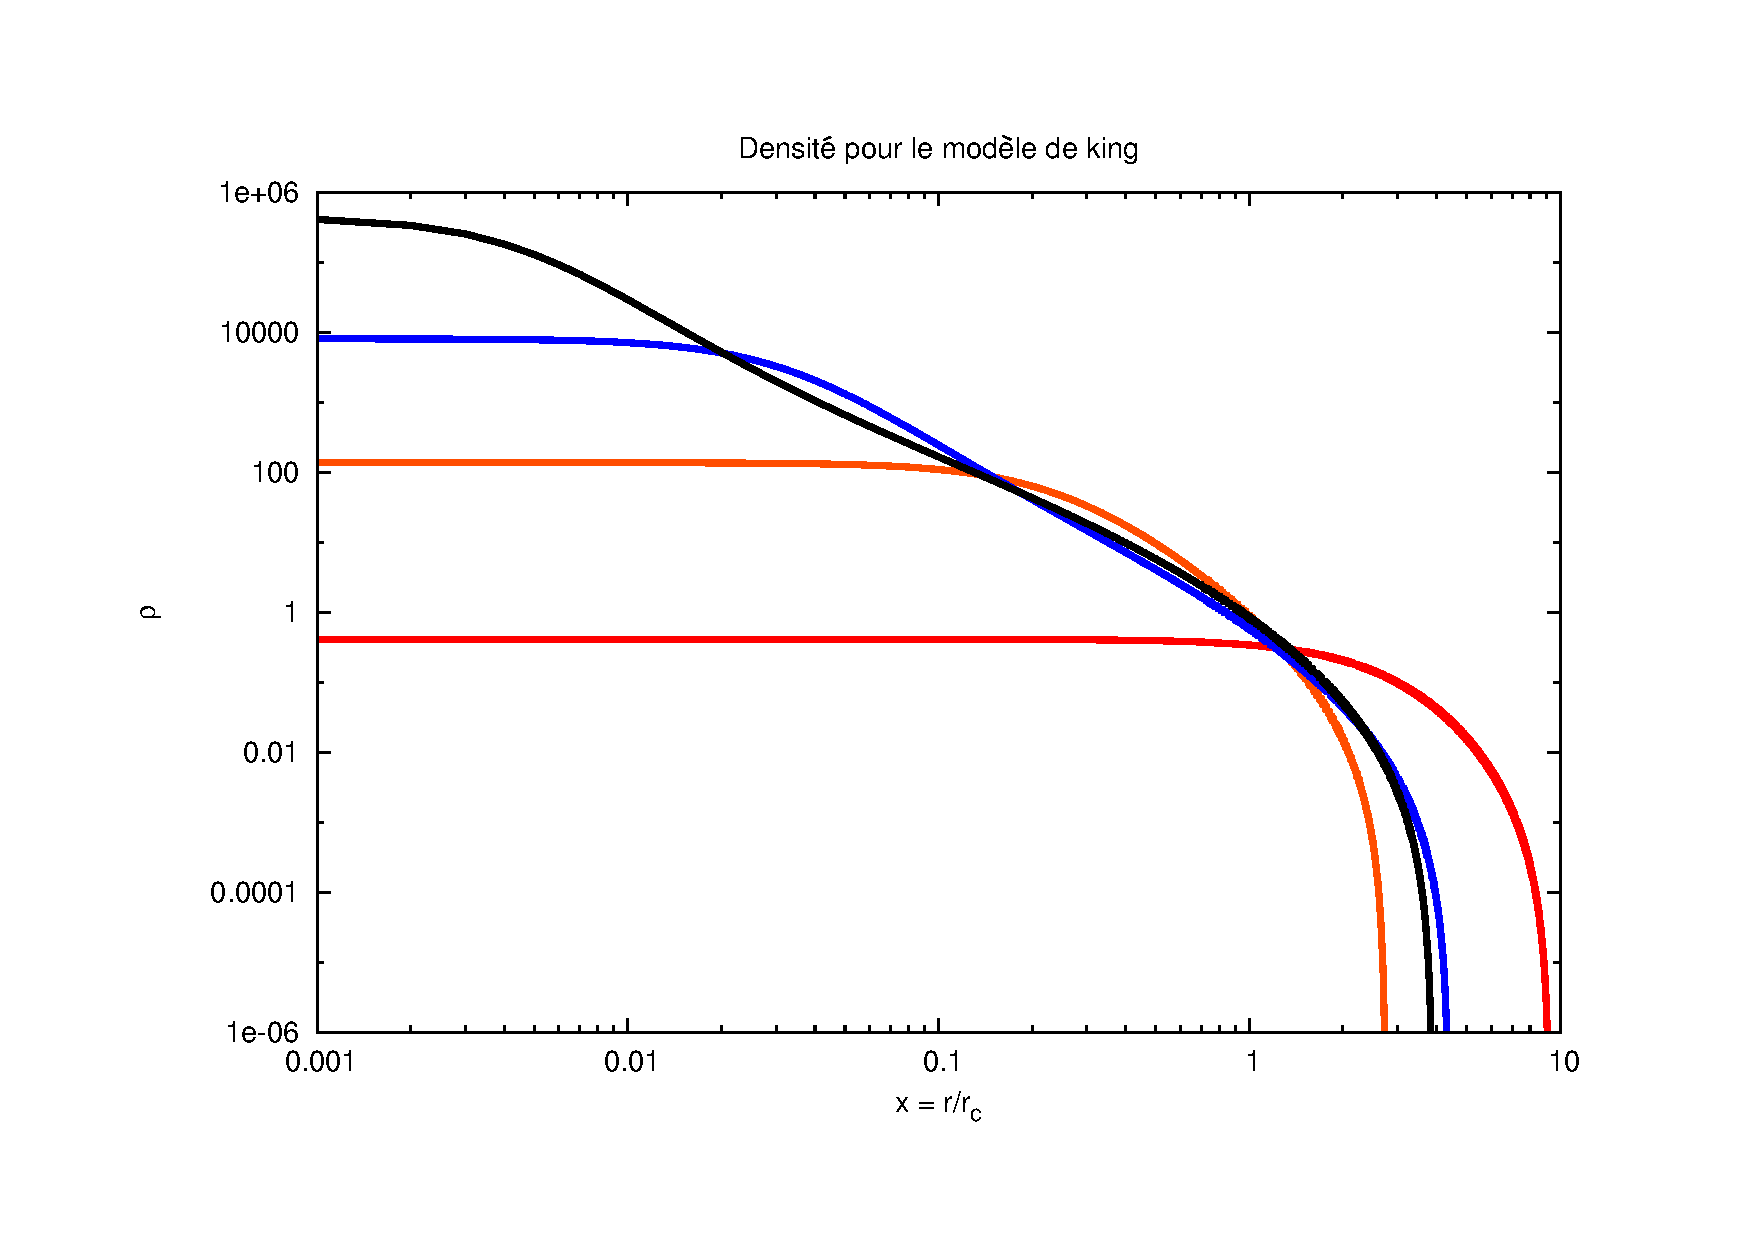
\includegraphics[width=\linewidth]{graphe/densite_pluri_limite-king_bis-4.pdf} };
						\draw[->, line width=1mm, visible on=<2->] (-0.5, 0.5) node[right] {$r_c$} -- (-0.9, -0.2);
						\draw[->, line width=1mm, visible on=<1->] (-4.5, 0.5) node[left] {$W_0$} -- (-3.5, -0.2);
						\draw[->, line width=1mm, visible on=<1->] (1, 0) node[above] {$W_0$} -- (0.4, -0.7);
						\draw[->, line width=1mm, visible on=<3->] (4.0, -5.5) node[below] {$E_l$} -- (4.0, -4.6);
					\end{tikzpicture}
					\note[item]<1->{En augmentant le paramètre $W_0$, on augmente la densité centrale et la pente $\Rightarrow$ on vieilli l'amas.}
					\note[item]<2->{En jouant sur ce paramètre, nous influons sur la largeur du puit de potentiel}
					\note[item]<3->{En jouant sur le dernier paramètre, c'est sur la taille de l'objet que l'on agit.}
					% \note<2>{En jouant sur ces paramètres, on peut alors influer très facilement sur la pente, la densité du cœur et son rayon.}
					% Mettre des labels aux fleche et les déplacer correctement.
					
					% New slides. Mettre des fléche pour indiquer influence des paramètres.
				\end{figure}
			\end{frame}
			\begin{frame}
				\frametitle{Modèle quasi-isotherme}
				\begin{figure}
					% \centering 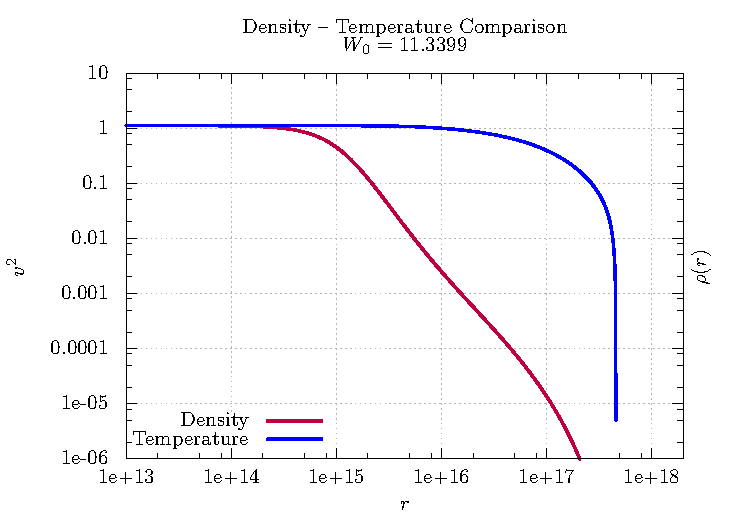
\includegraphics[scale=0.70]{graphe/temperature_11-3399_3.pdf}
					\centering 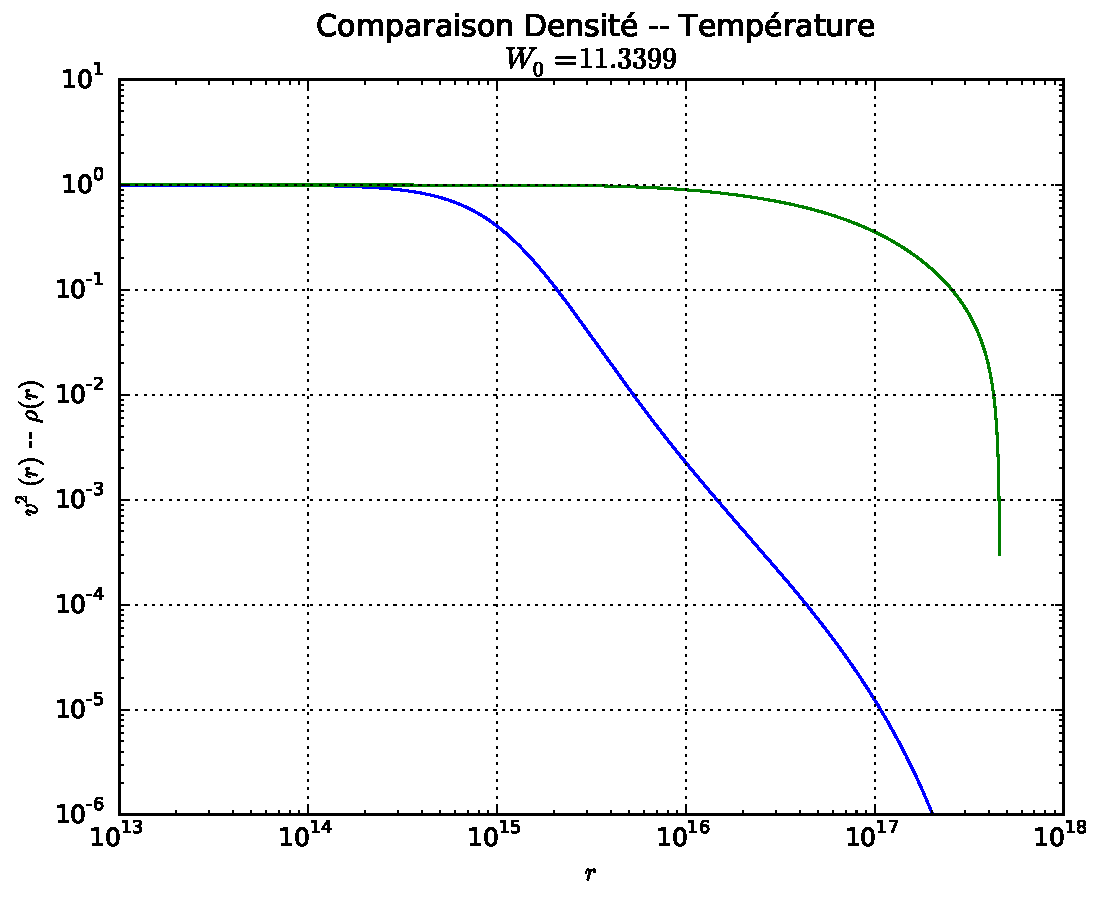
\includegraphics[width=0.8\linewidth]{graphe/densite-temperature2.pdf}
					\note{de plus ce modèle est isotherme! En effet, vous avez ici tracé en bleu la densité en vert la température. On voit que la température reste constante au niveau du cœur et commence à s'éloigner de 
					cette constante lorsque la densité est suffisamment faible pour rendre ceci négligeable.}
				\end{figure}
			\end{frame}
		\subsection{Sphère isotherme en boîte}
			\begin{frame}[t]{Sphère isotherme en boîte}
				\note{Le modèle de King a été introduit en appliquant une troncature en énergie à la fonction de distribution de la sphère isotherme. Nous allons maintenant voir le modèle de la sphère isotherme en boîte.\par}
				\note{Pour ce modèle, ...}
				\begin{block}{3 paramètres}
					\begin{enumerate}
						\item<1->[$R$] le rayon
						\item<2->[$H$] l'énergie
						\item<3->[$T$] la température
					\end{enumerate}
				\end{block}
				\note{On a deux possibilités intéressantes pour les CL:}
				\begin{minipage}[c][0.5\textheight][c]{0.45\textwidth}
					\only<4->{
						\begin{block}{Ensemble canonique}
						
						\begin{center}
							\begin{tikzpicture}[scale=1]
								\draw (0, 0) circle (1) (0, 0) node {$R$, $T$, $H$};
								\node at (0, -1.7) {$T=\text{cte}$}; %Bain thermique: $T=\text{cte}$};
							\end{tikzpicture}
						\end{center}
						\end{block}
						\note<4->{$T=\text{cte}$ => Micro canonique\par}
					}
				\end{minipage}\hfill
				\begin{minipage}[c][0.5\textheight][c]{0.45\textwidth}
					\only<5->{
						\begin{block}{Ensemble micro-canonique}

						\begin{center}
							\begin{tikzpicture}[scale=1]
								\draw (0, 0) circle (1) (0, 0) node {$R$, $T$, $H$};
								\node at (0, -1.7) {$H=\text{cte}$}; %Énergie conservée: $H=\text{cte}$};
							\end{tikzpicture}
							
							% \begin{tikzpicture}[scale=1]
								% \draw[fill=white] (0, 0) circle (1) (0, 0) node {$R$, $T$, $H$};
								% \node at (0, -1.7) {Ensemble micro canonique: $H=\text{cte}$}; %Énergie conservée: $H=\text{cte}$};
							% \end{tikzpicture}
						\end{center}
							\end{block}
						\note<5->{$H=\text{cte}$ => canonique\par}
					}
				\end{minipage}
			\end{frame}
	\section{Les instabilités}
	\begin{frame}{Sommaire}
		\note{Maintenant que nous avons vue les principaux modèles permettant de modéliser les SAG, nous allons nous intéresser aux différentes instabilité gravitationnelles pouvant influencer l'évolution des SAG. Nous commencerons pas l'instabilité d'Antonov,
		puis l'instabilité de Jeans et enfin l'instabilité d'orbite radiale.}
		\small \tableofcontents[currentsection, hideothersubsections]
	\end{frame}
		\subsection{L'instabilité d'Antonov}
			\begin{frame}[t]{L'instabilité d'Antonov}
				\begin{figure}
					\centering 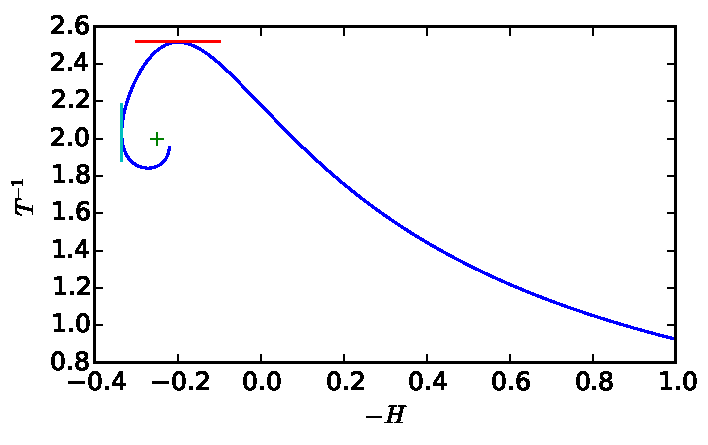
\includegraphics[width=1.\textwidth]{graphe/calorique_v2.pdf} %[scale=0.40]{graphe/sib_spirale2.pdf}
				\end{figure}
				\note{\scriptsize Une SIB ayant 3 paramètres, lorsque l'on trace T en fonction de H pour une valeur de R donnée, on obtient la courbe bleu. Lorsque l'on augmente R, on se déplace sur la spiral pour
					tendre asymptotiquement vers la croix verte représentant la sphère isotherme singulière. \par}
				\note{On remarque sur cette courbe que toute les valeur de la température ne sont pas accessible, idem pour l'énergie. Celle de la température sont limité par la tangente rouge, celle de l'énergie
					le sont par la tangente bleu.\par}
				\note{Ces tangentes correspondent à des instabilités. Si nous nous plaçons dans le cadre de l'ensemble canonique, nous pouvons imposer n'importe quel valeur de température à la SIB.
					Si cette valeur est trop faible, la SIB ne pourra pas retourner sur la courbe bleu. Elle va alors tendre vers la croix verte: la sphère isotherme singulière, qui n'est plus limité en rayon.
					Cette dernière n'a pas de cœur. Le raisonnement est le même pour l'ensemble micro-canonique.}
				% \note{Un moyen efficace de se représenter les SIB, auxquelles s'appliquent cette instabilité, est la courbe calorique. En effet, si vous tracez la $T$ en fonction de l'$H$, on obtient la courbe bleu,
					% paramétré par le rayon $R$ -> quand on se déplace dans ce sens (montrer sur slides)
					% R augmente, et l'on tend asymptotiquement vers la croix verte correspondant à la sphère isotherme singuliére que je vous ai présenté un peu plus tôt.\par}
				% \note{On ne peut pas mettre n'importe quel sphère dans n'importe quel boîte, en effet, on ne peut explorer toutes les valeurs de la température: en dessous d'une certaine valeur, il n'y a plus de
				% sphère possible. Idem en Énergie. Ces valeurs correspondent à des instabilité -> c'est l'instabilité d'Antonov.\par}
				% \note{La tangente horizontale correspond à l'ensemble canonique.\par}
				% \note{La tangente verticale correspond à l'ensemble micro canonique.\par}
				% \note{Si on fixe une température trop basse => impossible -> instabilité\par}
			\end{frame}
			\begin{frame}
				\frametitle{L'instabilité d'Antonov}
				\begin{minipage}[b]{0.53\linewidth}
					\begin{figure}
						\centering 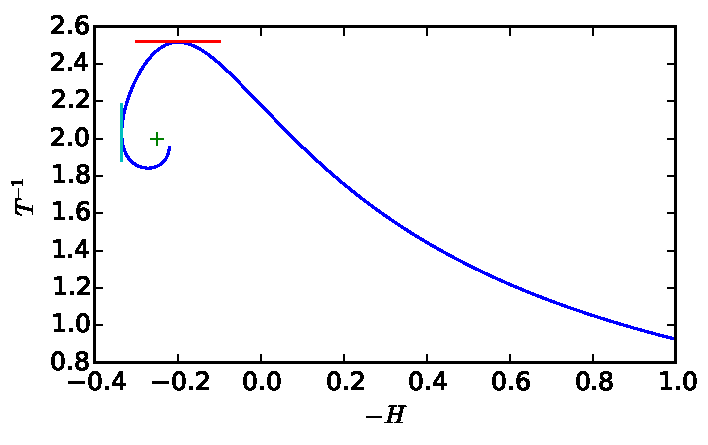
\includegraphics[width=1.\textwidth]{graphe/calorique_v2.pdf} %[scale=0.40]{graphe/sib_spirale2.pdf}
					\end{figure}
				\end{minipage}\hfill
				\begin{minipage}[b]{0.45\linewidth}
					$\qquad$\begin{tikzpicture}[scale=0.9]
						\draw (0.0,0.0) circle(2);
						\draw[red,very thick] (-0.5,1.0) -- (0.0,1.0) -- (1.0,-1.0) -- (1.28,-1.55);
						\draw (0.5,0) node[right]{$r^{-2}$};
						\draw (-0.5,0) node[right]{$T_{1}$};
					\end{tikzpicture}
				\end{minipage}
				\note{Le soucis étant que cette instabilités ne s'applique que au sphère isotherme en boîte, qui sont des objets présentant un profil cœur halo de pente $-2$. Or, nous avons vu que, si les SAG montre bien une structure cœur halo,
					la pente de leur halo est variable! De plus, le modèle de King, ayant une pente variable, est une bonne approximation d'une sphère isotherme!}
			\end{frame}
			\begin{frame}
				\frametitle{Instabilité d'Antonov généralisée}
				\begin{minipage}[b]{0.35\linewidth}
					\begin{figure}
						\centering 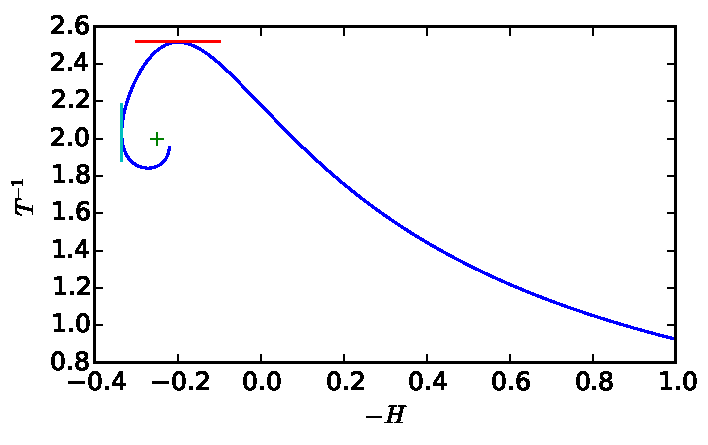
\includegraphics[width=1.5\textwidth]{graphe/calorique_v2.pdf} %[scale=0.40]{graphe/sib_spirale2.pdf}
						% \centering \includegraphics[scale=0.40]{graphe/sib_spirale2.pdf}
					\end{figure}
				\end{minipage}\hfill
				\begin{minipage}[b]{0.45\linewidth}
					\note{Nous avons donc étendu l'étude de l'instabilité d'Antonov à l'étude des systèmes cœur halo de pente quelconque dans le cadre de l'ensemble canonique.}
					\begin{center}
						\begin{tikzpicture}[scale=0.8]
							\draw (0.0,0.0) circle(2);
							\draw[red,very thick] (-0.5,0.5) -- (0.5,0.5) -- (0.75,-0.5);
							\draw (0.75,0.25) node[right]{$r^{-\alpha}$};
							\draw (-0.5,0) node[right]{$T_{1}$};
							\draw (2.7,0) node[right]{$T_{2}$};
						\end{tikzpicture}
					\end{center}
				\end{minipage}

			\end{frame}
			\begin{frame}
				\frametitle{Toy Model}
				\note{Nous avons représenté ici la courbe calorique pour plusieurs valeurs de la pente. La tangente horizontale, associée à l'instabilité d'antonov dans le cadre de l'ensemble canonique, est toujours présente! De tels objets sont donc
					toujours sujet à cette instabilité.}
				\begin{minipage}[b]{0.65\linewidth}
					\begin{figure}
						\centering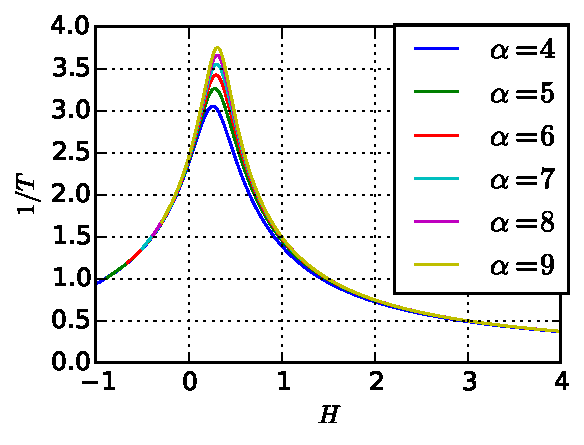
\includegraphics[width=1.0\textwidth]{graphe/Spirale_tm.pdf}
					\end{figure}
				\end{minipage}\hfill
				\begin{minipage}[b]{0.35\linewidth}
						\begin{tikzpicture}[scale=0.7]
							\draw (0.0,0.0) circle(2);
							\draw[red,very thick] (-0.5,0.5) -- (0.5,0.5) -- (0.75,-0.5);
							\draw (0.75,0.25) node[right]{$r^{-\alpha}$};
							\draw (-0.5,0) node[right]{$T_{1}$};
							\draw (2.7,0) node[right]{$T_{2}$};
						\end{tikzpicture}
					\hfill
					\hfill
					\hfill
				\end{minipage}
				% \note{Nous souhaitons généralisé cette étude à des obj de pentes quelconques afin de pouvoir l'appliquer à des
					% objets comme les SAG qui ont des pentes quelconques. De plus, les modèles de King ont des pentes
					% quelconques mais sont en plus quasi-isotherme.}
			\end{frame}
		\subsection{Instabilité de Jeans}
			\begin{frame}[t]{Instabilité de Jeans}
				\begin{minipage}[c][\textheight][c]{0.40\textwidth}
					\begin{center}
						\begin{tikzpicture}[scale=1]
							\draw[draw=none, shading=fadingdisk] (0, 0) circle (2) (0, 0); % node {$\rho_0$, $M$, $\sigma^2$};
						\end{tikzpicture}\\
						$\rho_0$, $M$, $\sigma^2$
					\end{center}
				\end{minipage}\hfill
				\begin{minipage}[c][\textheight][c]{0.40\textwidth}
					\visible<2->
					{
						\begin{tikzpicture}[scale=1]
							\pgfmathsetmacro{\ra}{0.3};
							\pgfmathsetmacro{\rb}{2.0};
							\pgfmathsetmacro{\n}{10};

							\draw[draw=none, shading=fadingdiskother] (0, 0) circle (\rb);
							\foreach \s in {1,...,\n} {
								\draw[->] ( {\rb * cos(360/\n * (\s - 1))}, {\rb * sin(360/\n * (\s - 1)} ) -- ( {\ra * cos(360/\n * (\s - 1))}, {\ra * sin(360/\n * (\s - 1)} );
							}
						\end{tikzpicture}
						\vspace{\toto}
					}
				\end{minipage}
				\note{L'instabilité de Jeans arrive lorsque l'on s'interesse aux boules homogénes: si l'on prend une boule homogène de densité $\rho_0$, de masse $M$ et de température $\sigma^2$, si la température cinétique n'est pas
					suffisamment importante pour contre balancer la pression gravitationnelle, cette boule va s'effondrer sur elle-même. C'est l'instabilité de Jeans. La théorie autour de cette instabilité ne nous dit pas quel
					est le profil résultant de cette effondrement, mais les simulations numérique nous apprennent que le résultat est une structure cœur halo de pente $-4$.}
			\end{frame}
		\subsection{Instabilité d'orbite radiale}
			\begin{frame}{Instabilité d'orbite radiale}
				\begin{minipage}[c][0.4\textheight][c]{\textwidth}
					\begin{tikzpicture}
						\pgfmathsetmacro{\rin}{0}
						\pgfmathsetmacro{\rmid}{0.5}
						\pgfmathsetmacro{\rout}{1}
						\pgfmathsetmacro{\astart}{20}
						\pgfmathsetmacro{\aend}{70}
						\pgfmathsetmacro{\atip}{10}

						\pgfmathsetmacro{\first}{0.6}
						\pgfmathsetmacro{\pas}{0.4}

						\fill[red, draw = red!50!black, very thick] (0, \rin) -- (\atip, \rin) -- (\atip + 0.5, \rmid) -- (\atip, \rout) -- (0, \rout) -- (0.5, \rmid) -- cycle;

						\draw[->, thick, visible on=<1->] (\first, \rout) -- (\first, \rin - 0.5) node[below] {\color{blue!85}{1973}};
						\draw[->, thick, visible on=<2->] (\first+8*\pas, \rout) -- (\first+8*\pas, \rin - 0.5) node[below] {\color{blue!85}{1981}};
						\draw[->, thick, visible on=<3->] (\first+14*\pas, \rout) -- (\first+14*\pas, \rin - 0.5) node[below] {\color{blue!85}{1987}};
						\draw[->, thick, visible on=<5->] (\first+18*\pas, \rout) -- (\first+18*\pas, \rin - 0.5) node[below] {\color{blue!85}{1991}};

						\draw[->, thick, visible on=<4->] (\first+13*\pas, \rin) -- (\first+13*\pas, \rout + 0.5) node[above] {\color{blue!85}{1986}};
						\draw[->, thick, visible on=<6->] (\first+21*\pas, \rin) -- (\first+21*\pas, \rout + 0.5) node[above] {\color{blue!85}{2004}};
						\draw[->, thick, visible on=<7->] (\first+23*\pas, \rin) -- (\first+23*\pas, \rout + 0.8) node[above] {\color{blue!85}{2009}};
					\end{tikzpicture}
				\end{minipage}

				\begin{minipage}[c][0.6\textheight][t]{\textwidth}
					\vspace{1cm}
					\only<1>{
						\begin{itemize}
							\item<1->[1973] Premier résultat analytique d'Antonov
							\note{la dernière instabilité est l'instabilité d'orbite radiale.\par}
							\note{Un système sphérique composé entièrement d'orbite radiale est instable et change de forme.}
						\end{itemize}
					}
					\only<2-3>{
						\begin{itemize}
							\item<2->[1981] Premier critère de stabilité (\emph{Polyachenko et Shukhman})%: $2\frac{E_c^r}{E_c^\perp} > 1.75 \pm 0.25$ pour $f\(E - \frac{\lambda L^2}{r_a^2}\)$
								\note[item]{Ils ont cherché un critère de stabilité en utilisant le pourcentage d'énergie appartenant à des orbites radiales.}
							\item<3->[1987] Il n'y a pas de critère de stabilité (\emph{Palmer et Papaloizou})%: $2\frac{E_c^r}{E_c^\perp} \approx 2.5$ pour $\rho(r) \propto (\frac{r}{r_0})^{-2}(1+\frac{r}{r_0})^{-2}$
								\note[item]{Mais une équipe anglaise montre, en étudiant plusieurs familles de modèle, qu'il n'y a pas de critère de stabilité simple:
								on peut avoir un système aussi anisotrope que l'on veut sans qu'il soit pour autant instable et inversement, on peut avoir un système aussi peu anisotrope sans qu'il soit pour autant stable.
								On commence à se rendre compte de la complexité de l'instabilité}
						\end{itemize}
					}
					\only<4>{
						\begin{itemize}
							\item[1986] Premières simulations sur IOR par \emph{Barnes et al.}
								\note{Entre temps, une équipe mené par barnes fait des simulations montrant l'apparition d'une barre comme produit de l'instabilité (Première apparition de la barre!)}
						\end{itemize}
					}
					\only<5>{
						\begin{itemize}
							\item[1987] {\color{blue!85}{\& 1991}} Première utilisation dans le cadre de la formation des structures cosmologiques (\emph{Merritt, 1987, Katz, 1991})
							\note{Merritt avec des simulations de formations de galaxies. Katz dans des simulations cosmologiques. Katz montre que le processus est tout de même gommé.}
						\end{itemize}
					}
					\only<6>{
						\begin{itemize}
							\item[2004] Nécessité d'un germe pour déclencher IOR (\emph{Roy et Perez})
							\note{Des simulations mettant en scène l'effondrement d'une boule homogène contenant des inhomogénéité ont montré que cette boule développait l'instabilité d'OR
								uniquement en présence des inhomogénéité. }%Montré à l'aide de simulation contenant des sphères (homogène ou non) imbriquées.}
						\end{itemize}
					}
					\only<7>{
						\begin{itemize}
							\item[2009] Instabilité dissipative (méthodes énergétiques) (\emph{Perez et Maréchal})
							\note{Ils ont montré que l'instabilité avait besoin d'un système à l'équilibre meta-stable pour pouvoir se déclencher.\par}
						\end{itemize}
					}
				\end{minipage}
				% \note{Cette instabilité e}
			\end{frame}
	\section{Simulations numériques}
	\begin{frame}{Sommaire}
		\note{Maintenant que nous avons en tête les principaux modèles et instabilités permettant de décrire l'évolutions des SAG, nous allons voir différents jeu de simulation que j'ai effectué au cours de ma thèse.}
		\small \tableofcontents[currentsection, hideothersubsections]
	\end{frame}
		\subsection{Motivation}
			\begin{frame}[t]{Expériences numériques}
				Objectifs:
				\begin{itemize}
					\item<1-> Reproduire les diverses instabilités
					\item<2-> Mettre en évidence certains mécanismes associés
				\end{itemize}
				\uncover<3->{Outils numérique principal:}
				\begin{itemize}
					\item<3-> Treecode public \textsc{Gadget-2} (Springel, 2005)
				\end{itemize}
				\uncover<4->{Validation:}
				\begin{itemize}
					\item<4-> Comparaison avec un code Vlasov
				\end{itemize}
			\end{frame}
			\begin{frame}[t]{Sphère de Hénon}
					\note{Au cours de nos simulations nous utiliserons comme conditions initiales des sphères de Hénon. Il s'agit d'une boule homogène dont les vitesses suivent une distribution gaussienne.\par}
					\note{Ces conditions initiales sont faîte pour s'effondrer sous l'effet de l'instabilité de Jeans. La vitesse de son effondrement est paramétré par le rapport du viriel $2E_c/E_p$.\par}
					\note{L'avantage de ces conditions initiales, c'est que leur effondrement produit un système très stable.}
				$$
					f(\vec{r}, \vec{v}) \propto \rho_0 e^{-\frac{\vec{v}^2}{2\sigma^2}}
				$$
				\begin{minipage}[c][\textheight][t]{0.45\textwidth}
					\begin{block}{Avantage}
						Son effondrement produit un système très stable
					\end{block}
					\begin{block}{}
						$$\gamma = \dfrac{2E_c}{E_p}$$
					\end{block}
				\end{minipage}\hfill
				\begin{minipage}[c][\textheight][t]{0.45\textwidth}
					\begin{block}{Densité}
						\centering \begin{tikzpicture}[scale=1]
							\draw[->] (0, 0) -- (0, 2);
							\draw[->] (0, 0) -- (2, 0);
							\draw[blue!85, line width=0.1mm] (0, 1) -- (1.5, 1) -- (1.5, 0);
							\node[left] at (0, 1) {$\overline{\rho(r)}$};
							\node[below] at (1, 0) {$r$};
						\end{tikzpicture}
					\end{block}
					
				\end{minipage}\hfill
			\end{frame}
		\subsection{Comparaison Vlasov-Gadget}
			\begin{frame}[t]{Comparaison Vlasov-Gadget: $\gamma=-0.5$}
				\only<1>{ \centering Condition initiale\\\centering \includegraphics[scale=0.55]{graphe/vlasov_gadget/{CompVlasGad_t_0_512_0.5}.png} }
				\only<2>{ \centering État intermédiaire\\\centering \includegraphics[scale=0.55]{graphe/vlasov_gadget/{CompVlasGad_t_13_512_0.5}.png} }
				\only<3>{ \centering État avancé\\\centering \includegraphics[scale=0.55]{graphe/vlasov_gadget/{CompVlasGad_t_45_512_0.5}.png} }
				\note<1>{Nous allons comparer un code résolvant l'équation de Vlasov avec un code Gadget. Le code Gadget est un code NCorps, et donc utilisant des particules pour
					représenter la fonction de distribution, qui utilise un code en arbre pour calculer les interactions entre particules. Pour minimiser les effets des collisions, il lisse la force.\par}
				\note<1>{Le code vlasov discrétise la fonction de distribution sur un maillage tridimensionnel utilisant comme variable le rayon, la vitesse radiale et le moment angulaire.\par}
				\note<1>{}
				
				\note<3>{L'accord reste remarquable tout du long de la simulation. Sur cette dernière image, nous y voyons un décalage temporel qui peut être dû aux paramètres de lissage ou pas de temps des codes.}
%% Éviter de se tirer une balle dans le pied. Cf thèse. Test paramètr...
			\end{frame}
			\begin{frame}[t]{Comparaison Vlasov-Gadget: $\gamma=-0.1$}
				\note{nous avons alors voulu pousser les limites des codes et donc faire la comparaison pour un effondrement plus violent. Là encore l'accord est remarquable!\par}
				\only<1>{ \centering Condition initiale\\\centering \includegraphics[scale=0.55]{graphe/vlasov_gadget/{CompVlasGad_t_0_512_0.1}.png} }
				\only<2>{ \centering État intermédiaire\\\centering \includegraphics[scale=0.55]{graphe/vlasov_gadget/{CompVlasGad_t_5_512_0.1}.png} }
				\only<3>{ \centering État avancé\\\centering \includegraphics[scale=0.55]{graphe/vlasov_gadget/{CompVlasGad_t_25_512_0.1}.png} }
				\note<3>{Jusqu'à la fin de la simulation où les codes montrent leurs limites. Le code Vlasov montre un nette effet de crénelage tandis que la simulation Gadget voit une instabilité se développer.\par}
				\note<3>{Cette instabilité ne dépend pas du paramètre de lissage de la force, ni du pas de temps. Par contre, il est possible de retarder son déclenchement en augmentant drastiquement 
				le nombre de particules. Cette instabilité est dûe aux effets collectif du bruit blanc des particules.}
			\end{frame}
		\subsection{Conditions Initiales}
			\begin{frame}
				\frametitle{Conditions Initiales}
%% J'AI FAIT !!!!!!!!!
%% Préciser nombre de simulations faîtes !
				\begin{exampleblock}{Bain thermique}
					Nous plongeons une sphère de Hénon dans un bain thermique
				\end{exampleblock}
				\note{On reprend une sphère de Hénon avec un viriel de $-0.5$. Cette sphère aura toujours les mêmes paramètres. On la plonge dans un bain thermique sous la forme d'un cube périodique.
					Le nb de particules, la taille du cube et la température du bain seront les paramètres de nos simulations.\par}
				\tikzstyle{every picture}+=[remember picture]
				\begin{minipage}[b]{0.30\linewidth}
					\begin{center}
						\begin{tikzpicture}
							\shade[shading=radial,inner color=white, outer color=red] (1.5,1.5) circle(1.5);
							\draw[blue,very thick] (1.0,1.5) -- (2.0,1.5);
							\path (3.0,1.5) coordinate (gauche);
						\end{tikzpicture}
					\end{center}
				\end{minipage}\hfill
				\begin{minipage}[b]{0.30\linewidth}
					\begin{center}
						\begin{tikzpicture}
							\shade[shading=radial,inner color=white, outer color=red] (1.5,1.5) circle(1.5);
							\draw[blue,very thick] (1.0,1.75) -- (2.0,1.75) -- (2.25,0.75);
							\draw (2.0,1.5) node[right]{$r^{-4}$};
							\path (0.0,1.5) coordinate (middle);
							\path (3.0,1.5) coordinate (middle2);
						\end{tikzpicture}
					\end{center}
				\end{minipage}\hfill
				\begin{minipage}[b]{0.30\linewidth}
					\begin{center}
						\begin{tikzpicture}
							\path (0.0,1.5) coordinate (droite);
							\shade[shading=radial,inner color=white, outer color=red] (1.5,1.5) circle(1.5);
							% \draw[blue,very thick] (0.5,2.0) -- (1.5,2.0) -- (2.0,0.5);
							\draw (1.5,1.5) node{?};
						\end{tikzpicture}
					\end{center}
				\end{minipage}
				\begin{tikzpicture}[overlay,decoration=zigzag]
					\path[->, black, thick] (gauche) edge[out=0,in=180] (middle);
					\path[->, black, thick] (middle2) edge[out=0,in=180] (droite);
				\end{tikzpicture}
				\note{Nous nous attendons, dans un premier temps à ce que la sphère de Hénon s'effondre pour donner une structure d'équilibre CH4.
				Ensuite, son évolution devrait être dictée par le bain et nous aimerions/nous attendons à voir l'une des deux autres instabilité décrite se produire.}
			\end{frame}
			\begin{frame}[t]{Une partie des simulations effectuées}
				\centering 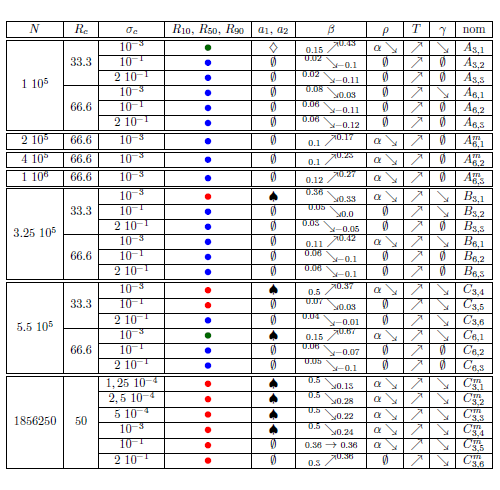
\includegraphics[height=0.8\textheight]{Table.png}
				\note{J'ai effectué près de 280 simulations, mais je n'en présenterais que 2 résumant bien les résultats obtenu.}
			\end{frame}
		\subsection{Instabilité d'orbite radiale}
			\begin{frame}[t]{L'instabilité d'orbite radiale décortiquée}
					\begin{minipage}{0.50\linewidth}
						\centering \includegraphics[width=\linewidth]{graphe/{ROI_radius_N-550000.0p1.5p1.5p1.5_Rc-33.3333333333p1.5_sc-0.001_Soft-0.001_new3}.pdf}
					\end{minipage}\hfill
					\begin{minipage}{0.50\linewidth}
						\centering \includegraphics[width=\linewidth]{graphe/{ROI_N-550000.0p1.5p1.5p1.5_Rc-33.3333333333p1.5_sc-0.001_Soft-0.001_new3}.pdf}
					\end{minipage}
					\begin{exampleblock}{}
						L'anisotropie: $\beta = 1 - \dfrac{\sigma_t^2}{2\sigma_r^2}$.\\
						$a_1$, $a_2$: les rapports des valeurs propres de la matrice d'inertie.
					\end{exampleblock}
					\note{\scriptsize{Nous avons à gauche les rayons à 10, 50 et 90\% de masse tracé au cours du temps. On y observe dans un premier temps l'effondrement de la sphère de Hénon pour former un état d'équilibre.}\par}
					\note{Après un petit temps, cette structure va commencer à accréter les particules du bain. Cette accretion se faisant de façon isotrope, l'objet voit son énergie cinétique radiale augmenter.
						C'est ce que montre le graphique de l'anisotropie radiale $\beta$ qui augmente au cours du temps.\par}
					\note{Cette accrétion commence sans déformer l'amas, comme nous l'apprend le graphique supèrieur droit qui montre l'évolution des rapports des valeurs propre de la matrice d'inertie.
					Au début de la simulation, ils sont proche de un => l'objet reste sphèrique. Puis il se déforme. Cette déformation est caractéristique/est la marque de l'instabilité d'orbite radiale.\par}
					\note{Nous voyions sur cette simulation toute les étapes que je vous ai décrit à propos de l'IOR: nous assistons à la formation d'un état d'équilibre qui va se déplacer vers la partie radiale de
					son espace des phases. Puis, lorsque cet équilibre devient méta stable, la dissipation associé aux interaction avec le bain le transforme en barre.\par}
					\note{D'autre simulations nous ont permit de montrer qu'il était possible de retarder ou de précipiter le déclenchement de cette instabilité en  jouant sur la densité du bain. La température de ce dernier ne semblant avoir que très peu d'effet }
			\end{frame}
			\begin{frame}[t]{Film}
				% \movie[externalviewer]{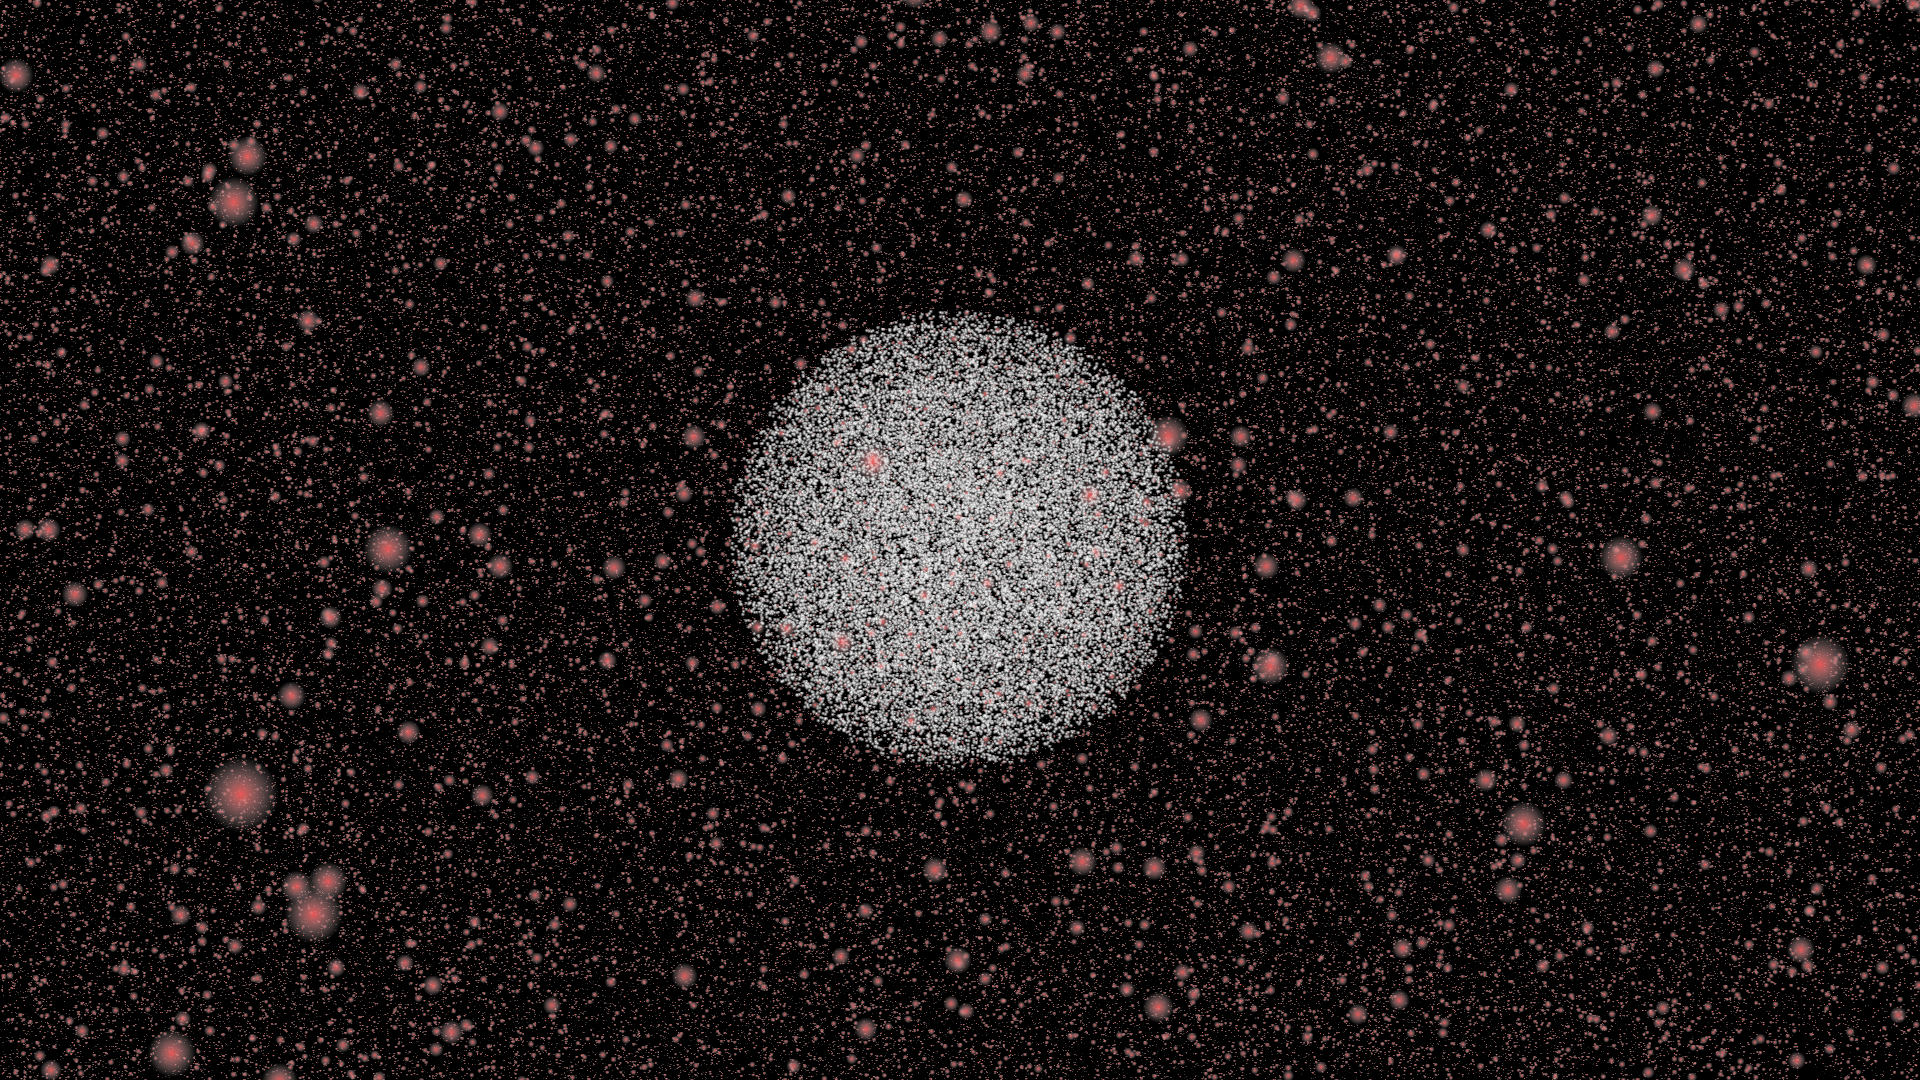
\includegraphics[width=\linewidth]{ROI_simu.png}}{ROI_simu.avi}
				\href{run:ROI_simu.avi}{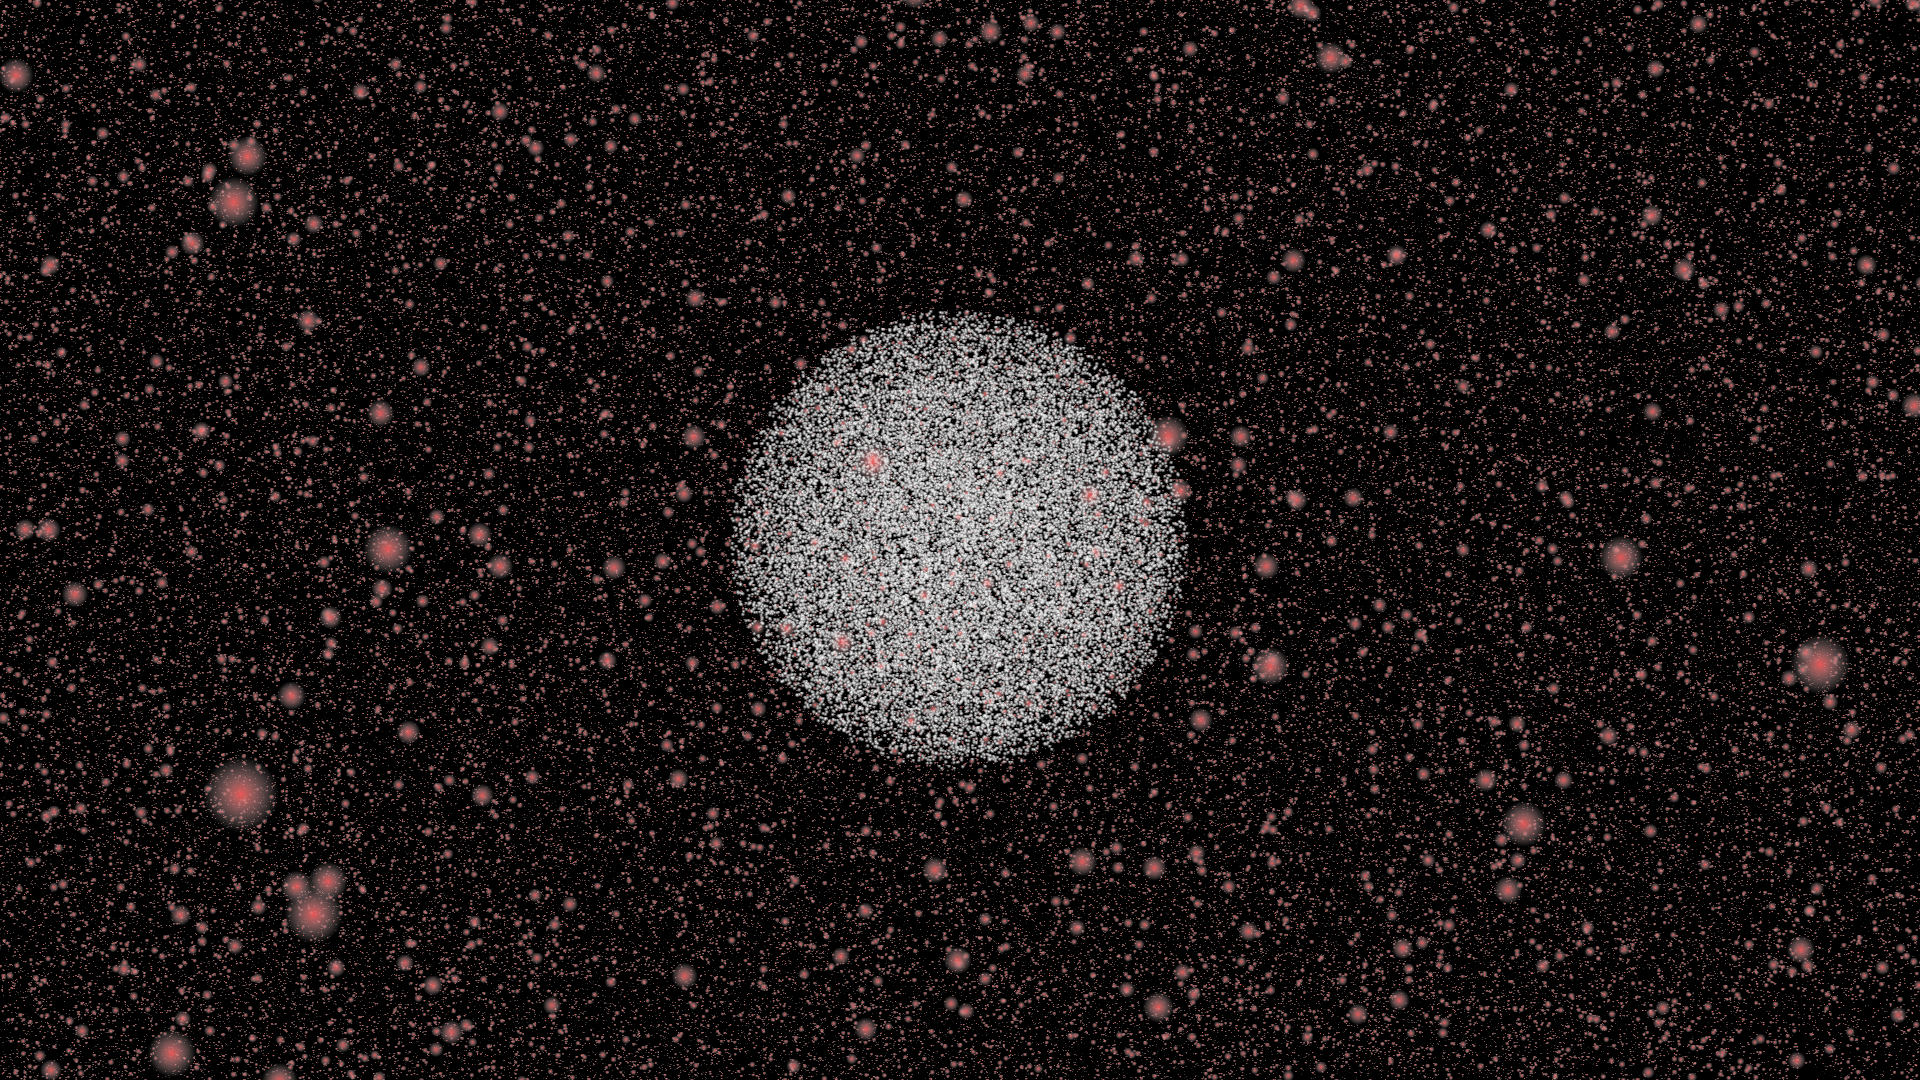
\includegraphics[width=\linewidth]{ROI_simu.png}}
				\note{Montrer le film tout en détaillant ce qui se passe.}
			\end{frame}
		\subsection{Effondrement gravitationnel}
			\begin{frame}[t]{Effondrement continu}
				\framesubtitle{Avec bain}
					\begin{tikzpicture}[overlay]
						\node at ($(current page.north west) + (0.4\paperwidth, -1.3\paperheight)$) { \includegraphics[width=0.8\linewidth]{graphe/{N-100000.0_Rc-66.6666666666_sc-0.001_evo_densityx1x2x4x10}.pdf} };
						\node at ($(current page.north west) + (0.4\paperwidth, -1.3\paperheight) + (-0.45, 3.)$) {$N=10^5$};
						\node at ($(current page.north west) + (0.4\paperwidth, -1.3\paperheight) + (3.12, 3.)$) {$N=2\ 10^5$};
						\node at ($(current page.north west) + (0.4\paperwidth, -1.3\paperheight) + (-0.3, -0.1)$) {$N=4\ 10^5$};
						\node at ($(current page.north west) + (0.4\paperwidth, -1.3\paperheight) + (3.0, -0.1)$) {$N=10^6$};
					\end{tikzpicture}
					\note{\scriptsize Nous en arrivons au second résultat important de nos simulations. Cette simulation a été effectué avec une densité du bain plus faible que pour la simulation précédente.
						Si le bain n'a aucun effet, nous nous attendons à ce que la structure résultant de l'effondrement de la sphère de Hénon n'évolue pas (comme sur le graphique en bas à droite).\par}
					\note{Or, dans notre simulation, cette structure continue à évoluer (voir le graphique en haut à gauche): sa densité centrale et la pente du halo continu continu à augmenter au cours
						de la simulation, tandis que son cœur tend à disparaître. Cette évolution n'est pas un effet du bain car, lorsque l'on augmente le nombre de particule de la simulation, cette tend à
						disparaître (voir sur les autres graphiques). Ceci suggérerait un effet des collision, mais la simulation c'est déroulée sur un temps équivalent à 20\% du temps de relaxation à 2 corps.\par}
					\note{Cette fois encore, il semblerait que l'effet soit dû au bruit collectif des particules. Ce mécanisme pourrait donc intervenir dans l'évolution des amas d'étoiles.}
					\note{Montrer le film, décrire en même temps. 1min grand max}
			\end{frame}
			\begin{frame}[t]{Effondrement continu}
					\begin{minipage}{0.50\linewidth}
						\centering 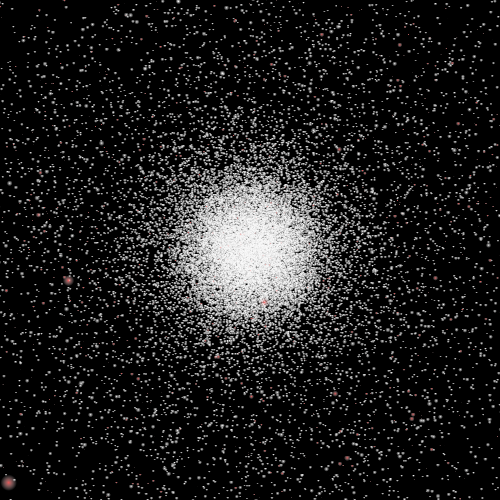
\includegraphics[width=\linewidth]{None_130.png}
					\end{minipage}\hfill
					\begin{minipage}{0.50\linewidth}
						\centering 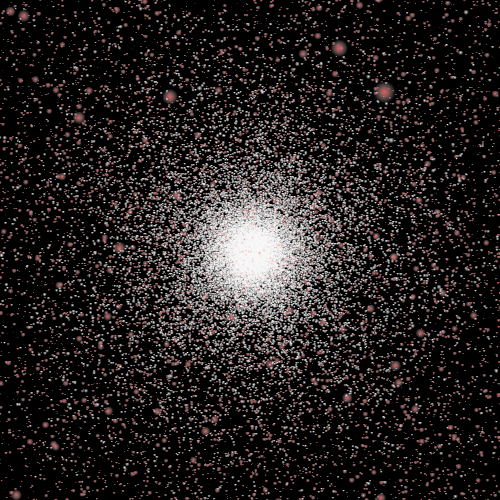
\includegraphics[width=\linewidth]{None_3000.png}
					\end{minipage}
					\note{en comparant ces images, nous voyons nettement que le cœur de l'objet à diminué.}
			\end{frame}
			\begin{frame}[t]{Effondrement continu}
					\note{ Cette évolution est similaire à celle que je vous ai décrite pour les amas, et les deux états que je viens de vous montrer ne sont pas sans rappeler $\omega$ du centaure et M15.}
					\begin{minipage}{0.50\linewidth}
						\centering 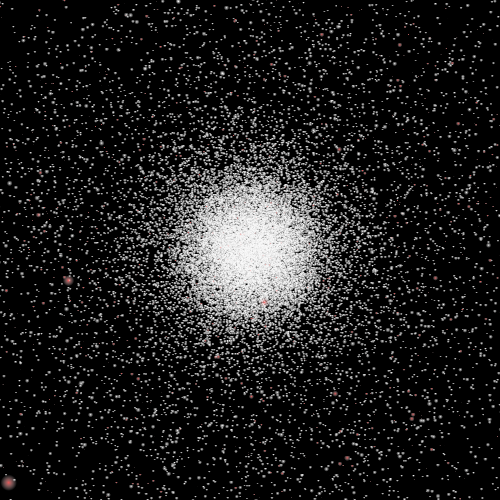
\includegraphics[width=0.7\linewidth]{None_130.png}
					\end{minipage}\hfill
					\begin{minipage}{0.50\linewidth}
						\centering 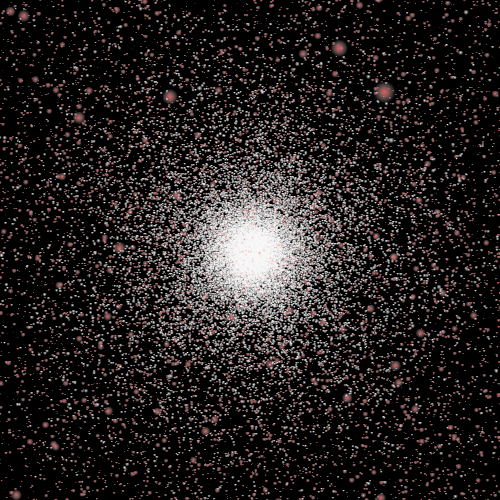
\includegraphics[width=0.7\linewidth]{None_3000.png}
					\end{minipage}
					\begin{minipage}{.5\linewidth}
						\centering 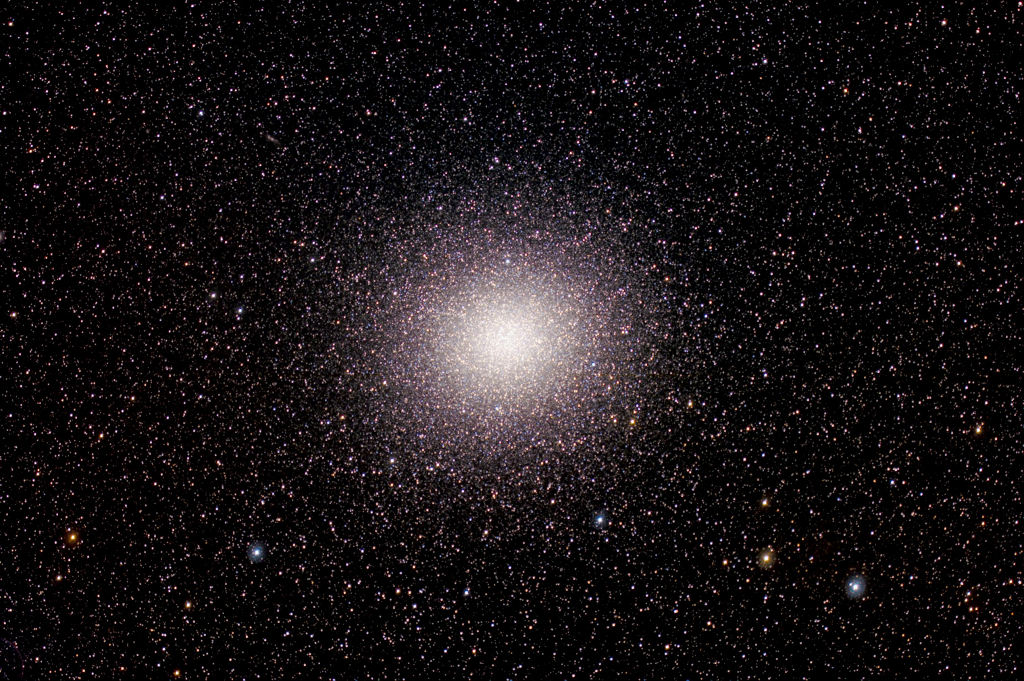
\includegraphics[width=0.7\linewidth]{graphe/ngc5139_w-cen_HD-2.png}
						% 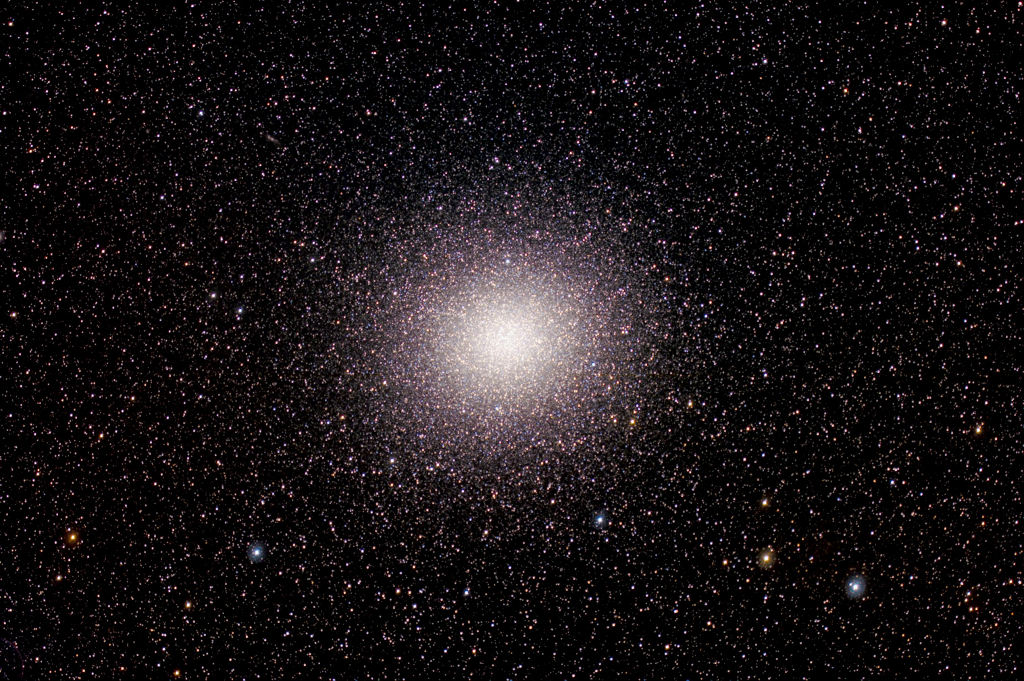
\includegraphics[scale=0.200]{graphe/ngc5139_w-cen_HD-2.png}
					\end{minipage}\hfill
					\begin{minipage}{.5\linewidth}
						\centering 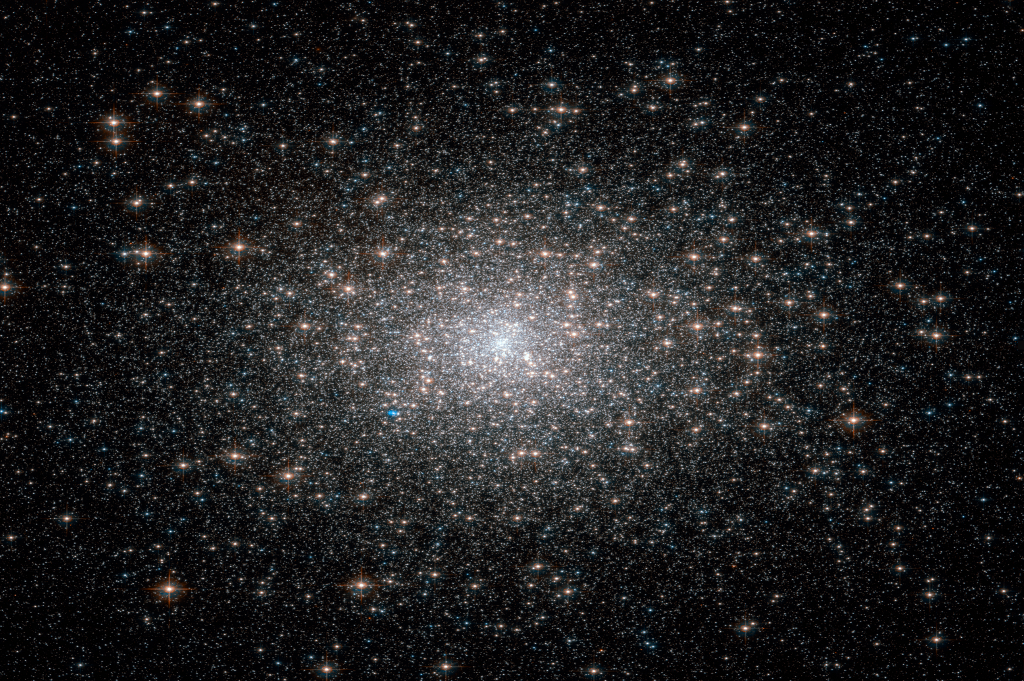
\includegraphics[width=0.7\linewidth]{graphe/m15_hst_4089_HD-2.png}
						% 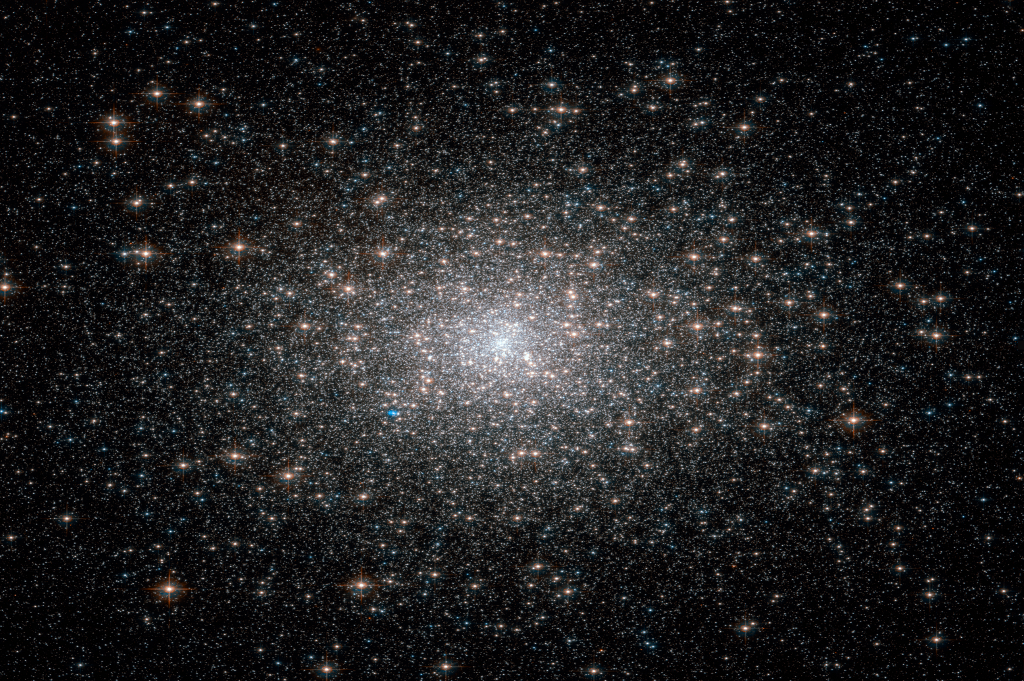
\includegraphics[scale=0.200]{graphe/m15_hst_4089_HD-2.png}
					\end{minipage}
			\end{frame}
			% \begin{frame}[t]{Effondrement suspect}
				% \framesubtitle{Sans bain}
				% % Sans bain:
				% \centering \includegraphics[width=0.8\linewidth]{graphe/{N-100000.0_Rc-66.6666666666_sc-0.001_evo_density_isox1x10}.pdf}
			% \end{frame}
	\section{Conclusions et perspectives}
		\begin{frame}[t]{Conclusions}
			\begin{block}{Amas globulaires}
				La pente du halo évolue avec l'âge.
			\end{block}
			\begin{block}{Instabilité d'Antonov}
				Généralisation de l'instabilité d'Antonov dans le cadre de l'ensemble canonique.
			\end{block}
			\begin{block}{Comparaison Vlasov-Gadget}
				Accord remarquable entre un code Vlasov et Gadget.
			\end{block}
		\end{frame}
		\begin{frame}[t]{Conclusions}
			\begin{alertblock}{Instabilité d'orbite radiale}
				\begin{itemize}
					\item[$\rightarrow$] Jeu de simulation mettant distinctement en évidence les diverses phases de l'instabilité.
					\item[$\rightarrow$] Dépendance du déclenchement avec la densité du bain.
				\end{itemize}
			\end{alertblock}
			\begin{exampleblock}{Un effondrement continu}
				\begin{itemize}
					\item Mise en évidence probable d'un nouveau mécanisme d'évolution de la structure coeur halo.
						%effondrement continu de la structure cœur halo.
					% \item Diverse explication
				\end{itemize}
			\end{exampleblock}

			% \begin{itemize}
				% \item Les SAG de type cœur halo sont de bonnes approximation des sphères isothermes.
				% \item Généralisation de l'instabilité d'Antonov.
				% \item Le déclenchement de l'instabilité d'orbite radiale est paramétré par la densité du bain.
				% \item Une simulation bizarre.
			% \end{itemize}
		\end{frame}
		\begin{frame}[t]{Perspectives}
			\begin{block}{Instabilité d'orbite radiale}
				\begin{itemize}
					\item \small{Étendre le domaine d'étude temporel des simulations pour raffiner l'influence de la densité du bain.}
					\item \small{Infirmer ou confirmer définitivement l'influence de la température du bain.}
				\end{itemize}
			\end{block}
			\begin{block}{Effondrement continu}
				\begin{itemize}
					\item \small{Étude de l'influence des paramètres du code Gadget-2 sur la simulation.}
					\item \small{Mise en place d'observables plus adaptées pour étudier la dynamique fine du système.}
				\end{itemize}
			\end{block}
			\begin{block}{Instabilité d'Antonov généralisée}
				\small{Augmentation de la densité ou de la température du bain.}
			\end{block}
		\end{frame}

		\begin{frame}[t]{Fin}
			% \Large\centering Fin!!!\par

			\begin{block}{}
				\centering Merci de votre attention!
			\end{block}
		\end{frame}

\end{document}

% vim: spelllang=fr
